This section highlights the key aspects of the event reconstruction which allow for the classification of neutrino interactions: track and shower reconstruction, particle identification (PID), and energy reconstruction.

\subsection{Track and Shower Reconstruction}
\label{sec:tkshreco}
The output of Pandora~\cite{bib:pandoraub} is organized in a hierarchy of reconstructed Particle Flow Particles (``PFParticles''), which describes the particle content in an observed event as a parent-daughter relationship chain. Final state PFParticles are 3D objects matching clusters of hits in at least two different planes.
Pandora classifies PFParticles as track-like or shower-like based on a Support Vector Machine (SVM) algorithm~\cite{bib:tkshsvm}, which produces a score with values between 0 (shower-like) and 1 (track-like). PFParticles will be collected together based on physical proximity into slices, and ordered into a hierarchy (i.e. a Michel electron is the daughter of a muon, which is a daughter of a neutrino).

Pandora processes track-like PFParticles with a sliding linear fit procedure (described in~\cite{bib:pandoraub}) that returns the 3D position and direction at each point along the trajectory, where each point corresponds to a 2D hit. 
For each point the \dqdx and distance from the track-start position are recorded using MicroBooNE's calorimetry module. 
This procedure makes it possible to accurately measure both d$x$, including small deflections due to the particle's trajectory, and space charge effect (SCE) offsets, as well as d$Q$, by incorporating MicroBooNE's full position- and field-dependent relative and absolute charge calibration. 
For tracks, the conversion from \dqdx to \dedx is performed by applying the inverse modified box recombination model~\cite{bib:tpccalibrationnote} with an electric field value obtained from MicroBooNE's position-dependent E-field map~\cite{bib:SCEdata}.

We evaluate the energy and 3D direction of shower-like PFParticles with the same algorithm used in the $\pi^0$ reconstruction paper~\cite{bib:pi0reco}. The energy reconstruction accounts for various detector effects, including gain and recombination. Corrections for reconstruction effects such as hit threshold and imperfect clustering will be described in Sec.~\ref{sec:ereco}. Showers are fit using a Kalman filter-based procedure~\cite{bib:shrtrackfitter} which aims to identify the main trunk of the shower by rejecting hits that are longitudinally or transversely displaced from it; the output of this fit is a track object which allows to use the calorimetric tools described above in order calculate precise 3D calorimetric information which accounts for the full calibrations developed by MicroBooNE. An important caveat needs to be pointed out: the conversion from \dqdx to \dedx is different for showers and tracks. For showers, both in the calculation of the trunk \dedx and in the total energy, we do not use a function that depends on the measured \dqdx value but we instead assume a constant recombination correction, compatible with the expected \dedx of 2.1 MeV/cm for MIPs. In all cases, local variations in the electric field are taken into account.

By default, Pandora separates showers and tracks with a cut on the SVM score at 0.5, however, as will be described in later sections, in many cases we choose different cut values, such as tighter shower definitions for the $\nu_e$ selection and looser for the $\pi^0$ control region.

The efficiency of Pandora's reconstruction on $\nu_e$ interactions is shown in Figure~\ref{fig:nuereco:eff} as a function of true neutrino energy. The efficiency for identifying the $\nu_e$ events as neutrino interactions is shown in black, and the efficiency for reconstructing $\nu_e$ interactions with a final-state EM shower in blue. The efficiency has a sharp upturn between 100 and 200 MeV, especially in the case when an EM shower is required, and levels off at 80\% and 60\% respectively for the two curves. 
\par At this stage in the analysis, the good efficiency for reconstructing $\nu_e$ events is offset by the very low signal-to-background for $\nu_e$ events in MicroBooNE's data, which is a consequence of the very small $\nu_e$ content of the beam. With no additional requirement on the reconstructed neutrino, the purity for $\nu_e$ interactions is 0.12\% (figure~\ref{fig:nuereco:sliceid}). After imposing a requirement of one reconstructed shower, the purity grows by almost an order of magnitude, to 1\% (figure~\ref{fig:nuereco:shower}). The $\nu$ background composition also changes significantly, with $\pi^0$ backgrounds moving from 14\% to 48\% of all backgrounds.

\begin{figure}[H] 
\begin{center}
    \begin{subfigure}[b]{0.3\textwidth}
    \centering
    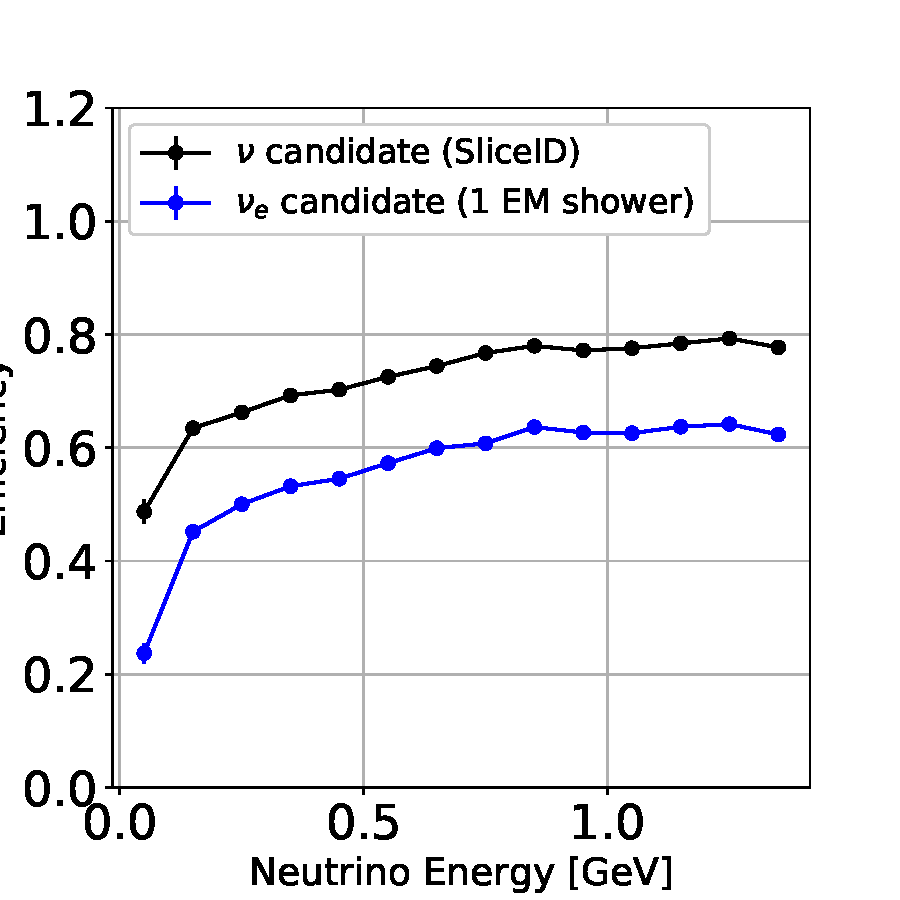
\includegraphics[width=1.00\textwidth]{nureco/nureco_RUN1.pdf}
    \caption{\label{fig:nuereco:eff} $\nu_e$ reconstruction efficiency}
    \end{subfigure}
    \begin{subfigure}[b]{0.31\textwidth}
    \centering
    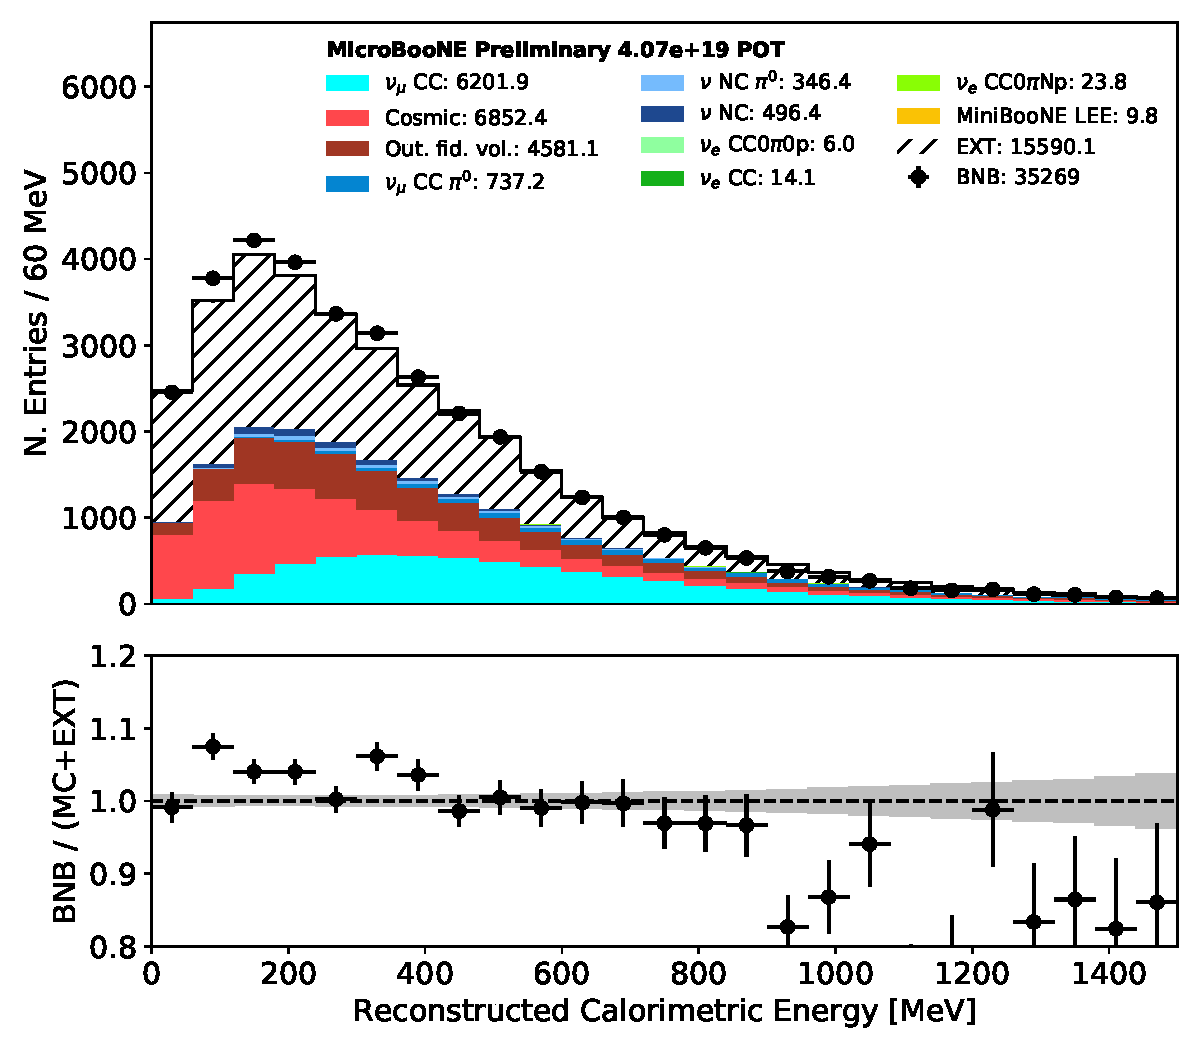
\includegraphics[width=1.00\textwidth]{nureco/NeutrinoEnergy2_01152020.pdf}
    \caption{\label{fig:nuereco:sliceid} After \texttt{SliceID}}
    \end{subfigure}
    \begin{subfigure}[b]{0.31\textwidth}
    \centering
    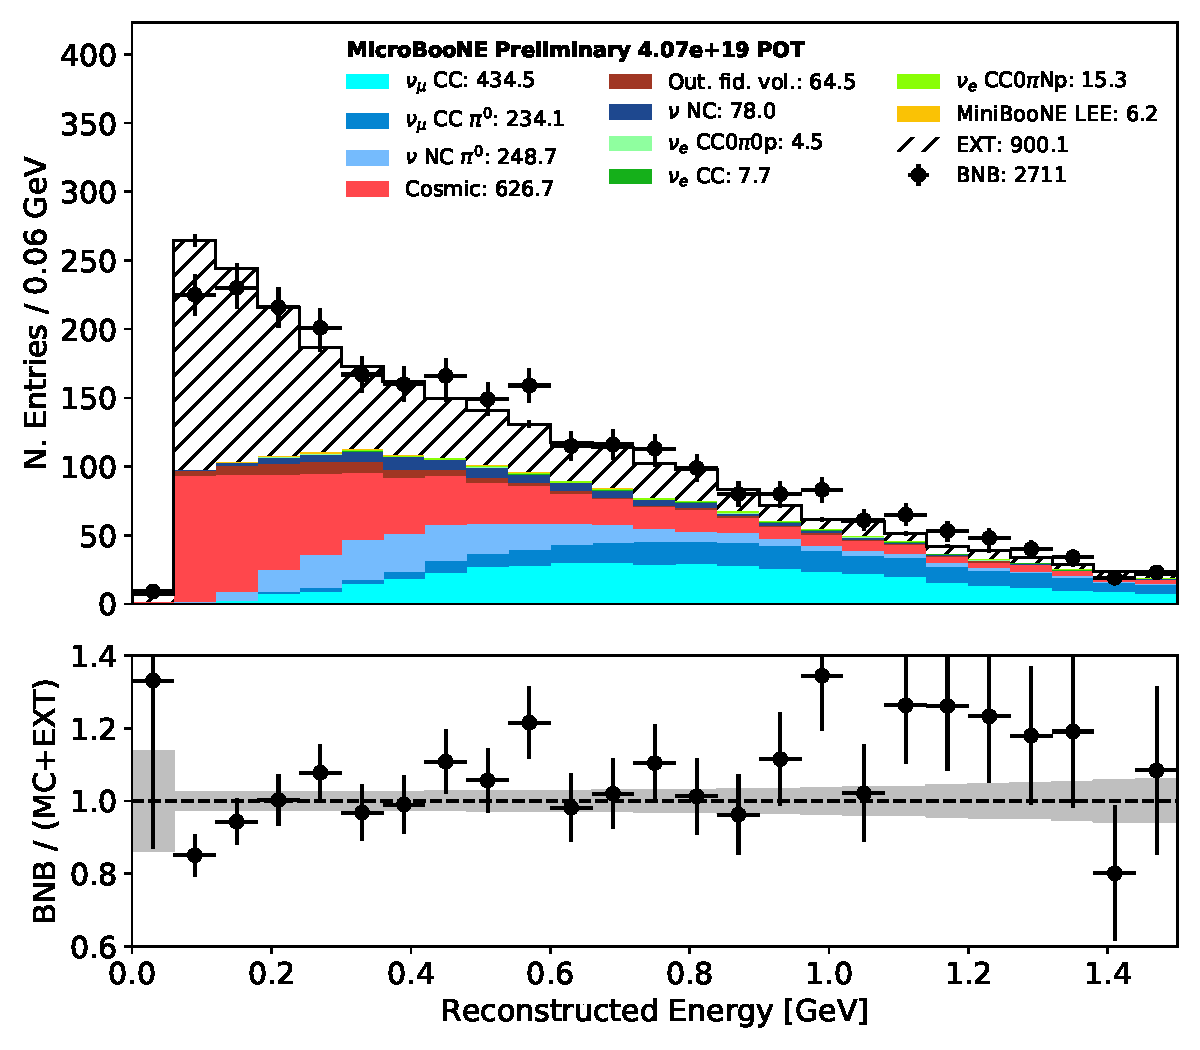
\includegraphics[width=1.00\textwidth]{nureco/reco_e_01152020.pdf}
    \caption{\label{fig:nuereco:shower} After shower requirement}
    \end{subfigure}
\caption{\label{fig:nuereco} a: Efficiency of the \texttt{SliceID} (black) and shower-requirement (blue) for $\nu_e$ events. b: data-MC comparison after \texttt{SliceID}. c: data-MC comparison after shower requirement. }
\end{center}
\end{figure}

\par The next step in the analysis requires the development of a selection capable of isolating $\nu_e$ interactions and rejecting the two order of magnitude larger background rates from $\nu_{\mu}$s. This selection will make use of PID and topological information described in the next sections. The strong level of background rejection needed to isolate signal events will inevitably lead to a lower selection efficiency.


\subsection{dQ/dx re-calibration}
\label{sec:recalibration}
The use of calorimetric information is essential in order to correctly identify different particles in the event.
Good data/simulation agreement in the \dedx distributions is necessary in order to ensure that PID-related cuts have the same impact on data and simulation.
Prompted by the observation of significant deviations in comparison of calorimetric information from calorimetric information, a re-calibration method has been developed in order to implement a correction of the simulation charge response to match the data. The only purpose of this re-calibration is to ensure data/simulation agreement.
In this re-calibration we compare the distribution of \dqdx between data and simulation using sample of cosmic muons in bins of angular variables, and derive multiplicative factors to be applied to the simulation to better match the data.

\paragraph{Selection of cosmic muons}
We consider a high-purity sample of cosmic MIP muons crossing the detector.
This is achieved by looking at the anode-cathode-piercing-tracks (ACPT)~\cite{bib:ACPT}, which are cosmic muons that cross the detector either through the anode or through the cathode.
%These cosmic rays can be identified by matching the flash time with the time of arrival of the charge under the hypothesis that it crosses the anode or the cathode.
These are cosmic rays for which $t_0$ is known and thus the full 3D trajectory coordinates are available.

For data, the Beam OFF sample is used. For simulation a standard overlay sample where an ACPT muon in the beam window is simulated using Corsika is used.
Tracks are required to be at least 20 cm long, and to be reconstructed as downward going. These last two requirements have an efficiency of 97\% in both data and simulation.

\paragraph{Data/simulation comparisons in angular bins}
The \dqdx along the ACPT tracks is compared between data and simulation, and a correction for the simulation is derived.
The main target of the re-calibration procedure is to ensure good data/simulation agreement for the track likelihood PID.
The main discrepancies we want to correct are related to the detector response, which includes all steps that bring the charge deposited in the detector to the reconstructed value of \dqdx.
Because the simulation of charge-loss and signal processing have a strong dependence on the angle at which a particle is travelling, we chose to derive corrections in bins of angular variables.
We use polar coordinates $\theta'$ and $\phi'$ with respect to the direction $z'$.
This is defined as the direction orthogonal to the wires and that lies on the wire plane.
These coordinates are defined plane by plane in a consistent way.
The prime is used to distinguish them from the usual MicroBooNE coordinate system, despite, for the collection plane, $z'$, $\theta'$, and $\phi'$ coincide with the usual $z$, $\theta$, $\phi$ in the detector.
In order to have a more intuitive parametrisation, we decided to shift from $\theta'$ to the pitch.
The pitch is the distance over which the charge measured in a hit has been deposited.
It is the quantity used as $\Delta x$ or $dx$ to estimate the \dedx associated with a hit\footnote{The expression for $dx$ used in this work, taken from the standard \texttt{Calorimetry} module employed in LArSoft, was checked to be consistent with the definition used in NIM A 498 (2003) 292–311, describing calorimetric reconstruction in ICARUS.}.
It depends on the local direction of the track with respect to the wire direction, and except for the small space charge correction, the pitch is a bijective function of the polar angle $\theta'$.
\[ \text{pitch} = \frac{0.3~\text{cm}}{|\cos(\theta')|} \]
In the end $\text{pitch}$ and $\phi'$ are the variables chosen to separate the different features of the \dedx distributions: the physical \dedx distribution from the peak at 0 MeV/cm, discussed in detail in section \ref{sec:particleid}.
The binning (five bins in pitch and six bins in $\phi$) is defined as follows:
\begin{itemize}
    \item $\text{pitch}$: $[0.3, 0.4, 0.7, 1., 1.5, 30]$ cm
    \item $\phi'$: $[0, 0.26, 0.52, 0.79, 1.05, 1.31, 1.57]$
\end{itemize}

Leveraging the symmetries of the detector geometry and specifically the chosen spherical coordinate system, we choose to consider only the magnitude of the direction components, which corresponds to defining:
\begin{equation}
\label{eq:phi}
\theta = \arccos{|u_z|} \quad \phi = \arctan{(|u_y|, |u_x|)}
\end{equation}
%It is important to stress that we consider only positive values of the pitch and $0 < \phi' < \pi/2$.
%Because of the symmetry of the detector, we believe that the response of the detector only depends on $|u_x|, |u_y|, |u_z|$, where $u_x$, $u_y$, $u_z$ are the Cartesian components of the direction vector in the rotated frame of the wire plane under consideration ($x$ is the drift direction, $y$ is the wire direction, $z$ is on the wire plane, perpendicular to every wire).
%In fact, by exploiting the symmetry of the detector, we bring the other values of pitch and $\phi'$ in this region.
%This is equivalent to doing the following:
%\[ \theta = \arccos{|u_z|} \quad \phi = \arctan{(|u_y|, |u_x|)} \]
%instead of 
%\[ \theta = \arccos{u_z} \quad \phi = \arctan{(u_y, u_x)} \]

Note that we compare the distribution of \dqdx rather than \dedx as the re-calibration tries to address data-MC discrepancies associated with measurements of drifting charge that are independent from possible effects of recombination mis-modeling.
As, within the context of a given ion recombination model, the measured \dedx is a bijective function of the measured \dqdx, the only difference between a correction factor on \dqdx or \dedx in the context of this analysis arises from the non-linearity of this function.

In each bin of pitch and $\phi'$, the best multiplicative scale factor is obtained through a binned maximum likelihood fit.
% An example is shown in Figure \ref{fig:recalibration_example} for the bin with 0.7 cm $<$ pitch $<$ 1 cm and 0.26 $< \phi' <$ 0.52.
% The left plot illustrates the likelihood scan and the best fit point.
Figure \ref{fig:recalibration_example} shows two examples of \dqdx distributions in the data compared to the simulation before and after the re-calibration is applied.
The agreement increases considerably, although the simulation is not perfect.
In an intuitive way, we can think of this as a correction of the scale of the distribution, whereas a correction of its width, through an additional smearing for example, is still missing.

\begin{figure}[H] 
\begin{center}
    \begin{subfigure}[b]{0.48\textwidth}
    \centering
    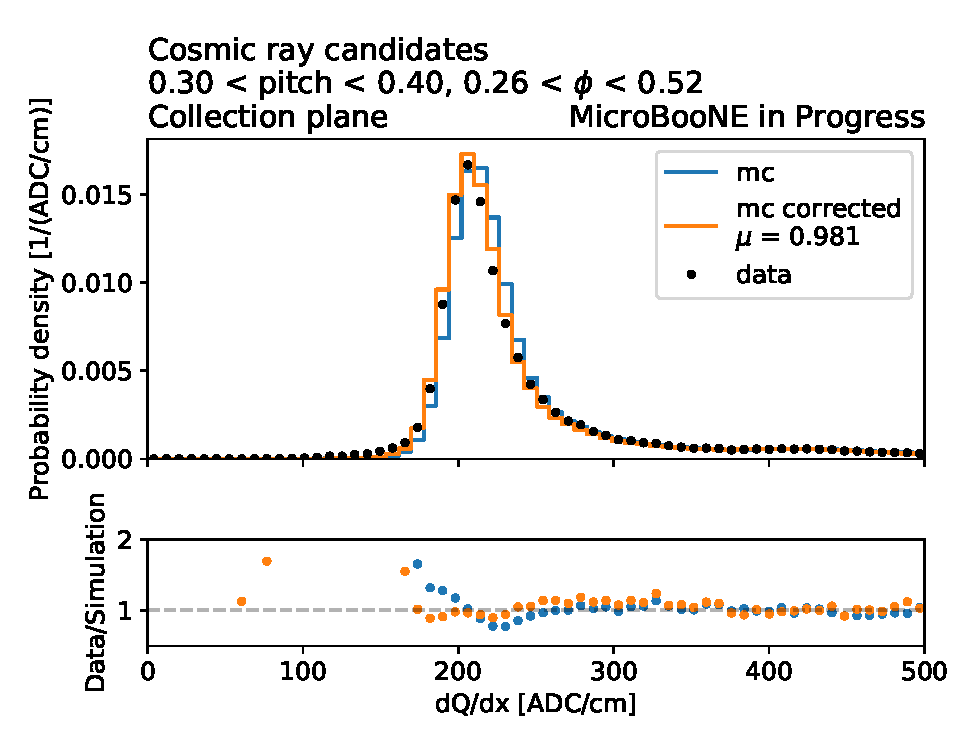
\includegraphics[width=1.00\textwidth]{recalibration/pitch_035_phi_039.pdf}
    \end{subfigure}
    \begin{subfigure}[b]{0.48\textwidth}
    \centering
    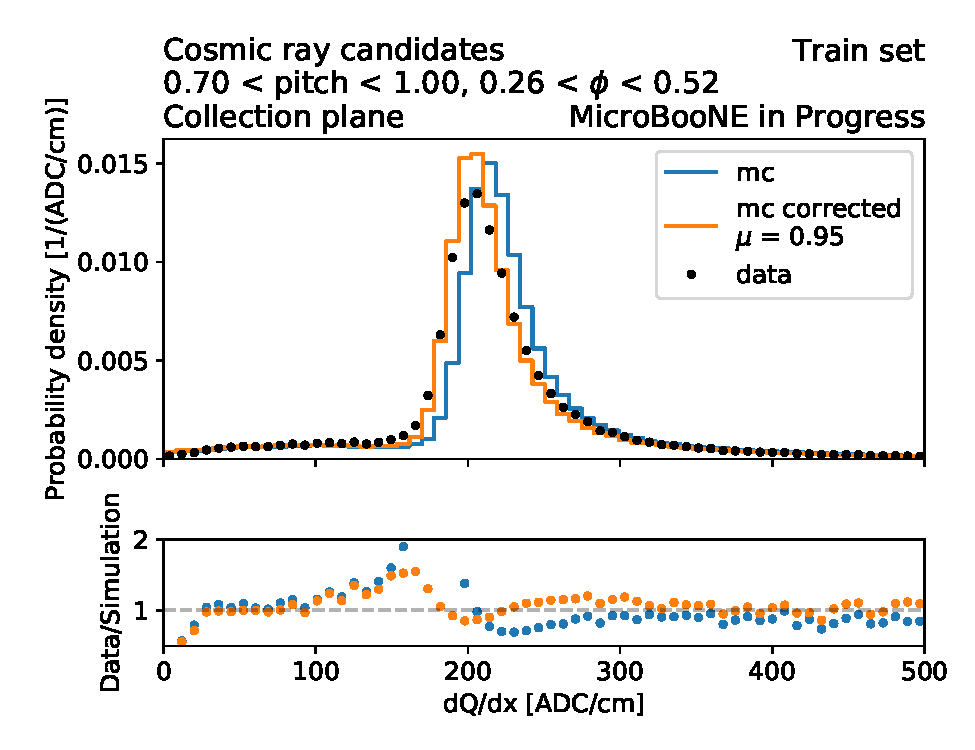
\includegraphics[width=1.00\textwidth]{recalibration/pitch_085_phi_039.pdf}
    \end{subfigure}
\caption{A maximum likelihood fit of the multiplicative correction factor is performed in bins of pitch and $\phi'$. 
The two plots show two examples of the \dqdx distributions in two different angular bins, comparing the data with the simulation before (blue) and after (orange) applying the correction.
}
\label{fig:recalibration_example}
\end{center}
\end{figure}

The re-calibration is summarised in the three tables shown in Figure \ref{fig:recalibration_tables}, for the three wire planes.
There is one more bin at very large pitch which is not included in the plots.
In each bin of pitch and $\phi'$, the multiplicative factor is shown.  Generally, we see smooth correction maps, indicating that we are not subject to statistical fluctiations in the computation of the re-calibration. The largest features observared are that on the induction planes the MC needs to be scaled up by up to 10\%, while on the collection-plane the MC needs to be scaled down by $\mathcal{O}$(3-4\%). Re-calibration factors tend to be larger at larger angles and pitch values.
The re-calibration is then applied to every measured value of \dqdx in the rest of the analysis for simulation-induced charge: for each calorimetry point, the corresponding 3D direction is used to compute the pitch and the angle $\phi'$, and the correction factor is read from the table.

\begin{figure}[H] 
\begin{center}
    \begin{subfigure}[b]{0.30\textwidth}
    \centering
    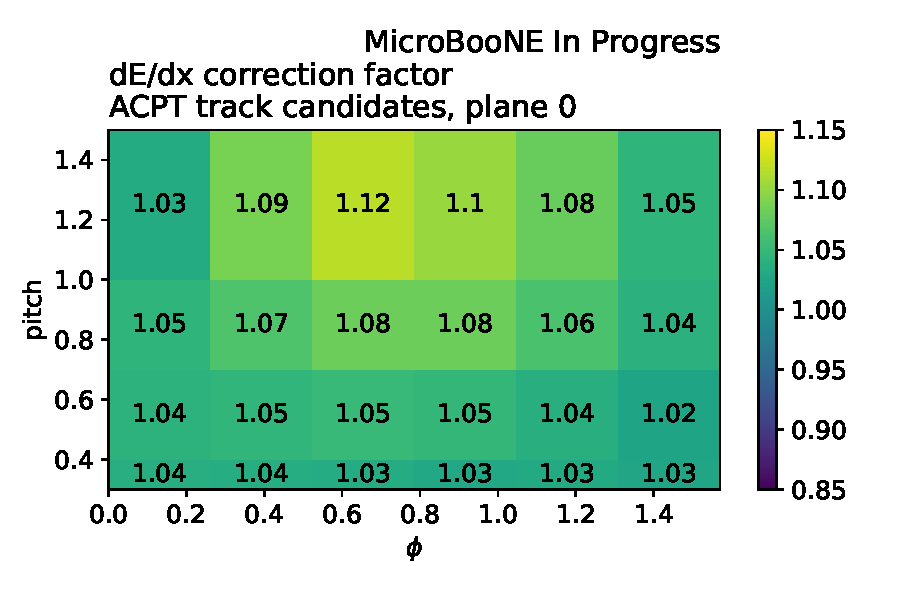
\includegraphics[width=1.00\textwidth]{recalibration/calibration_table_plane_0.pdf}
    \end{subfigure}
    \begin{subfigure}[b]{0.30\textwidth}
    \centering
    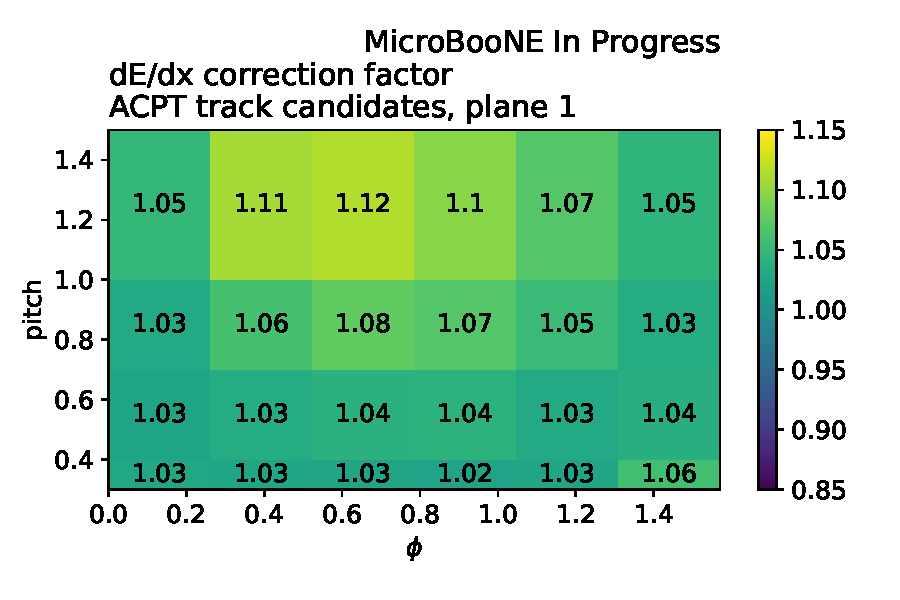
\includegraphics[width=1.00\textwidth]{recalibration/calibration_table_plane_1.pdf}
    \end{subfigure}
    \begin{subfigure}[b]{0.30\textwidth}
    \centering
    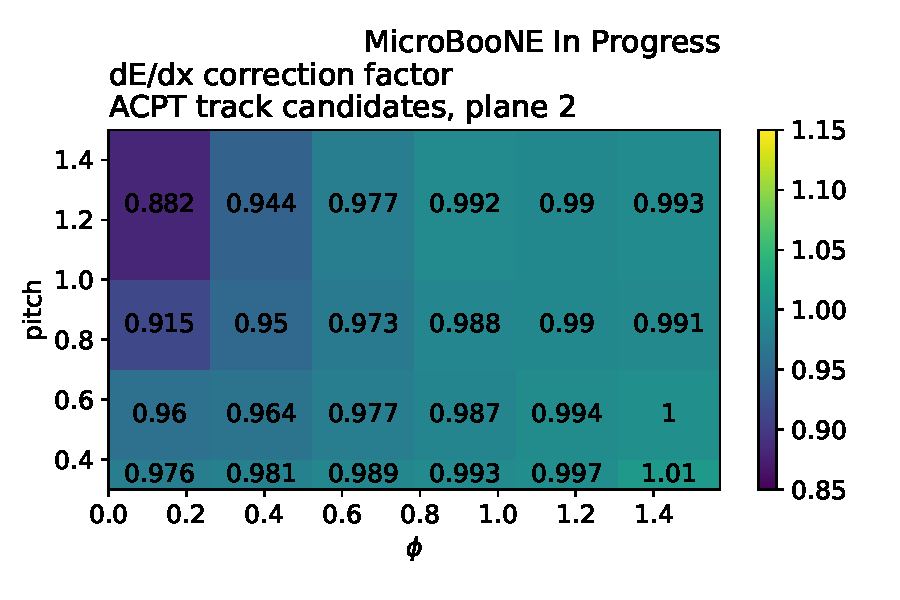
\includegraphics[width=1.00\textwidth]{recalibration/calibration_table_plane_2.pdf}
    \end{subfigure}
\caption{Re-calibration tables, showing the multiplicative factors in bins of pitch and $\phi'$, for the three wire planes.}
\label{fig:recalibration_tables}
\end{center}
\end{figure}

\paragraph{Remarks}
We finally describe the limitations of the developed re-calibration, along with the studies performed to assess their impact on the analysis.
The first limitation comes from having implemented a binned correction, developed with especially coarse bins. The bin width is dictated by the limited statistics of the samples. We checked that by decreasing the statistics in each bin, for example splitting the sample in train and test, we introduce statistical fluctuations that can cause biases in the correction.
Second, despite improving the agreement by aligning the \dqdx peaks in every bin, the correction is not perfect as it lacks an additional smearing effect due to mis-modeling of the charge resolution of the detector. A more complex correction accounting for such effects might be performed in a future iteration of this study.
Third, the observed discrepancies can in principle depend on additional variables, such as the position in the detector.
Including additional variables in a binned correction is not possible while preserving the necessary statistics needed for effective re-calibrations. Limitations to the re-calibration itself are covered by the wire-modification approach to TPC detector systematics employed by the collaboration.

Finally, while it is reasonable to expect that the detector response is uniform over a broad range of energy deposition values, this is not guaranteed. 
The behavior for shower-like objects may additionally differ from that of track-like objects.
For this reason a proper validation of the re-calibration has been developed using neutrino-induced muons and protons.
Some of these comparisons are shown in Section \ref{sec:sideband:stopping_muons_protons}. Comparisons for photon showers are included in Section~\ref{sec:sideband:pi0}.
The interested reader might find all details of the method and the validation in \cite{bib:pid_internal_note}.

\subsection{Particle Identification}
\label{sec:particleid}

Particle identification in this analysis focuses on $\mu$/$p$ separation for tracks, and $e$/$\gamma$ separation for showers. While the PID methods developed by the analysis rely on the same underlying calorimetric information obtained from track-fitted \dedx information, PID is performed with different tools depending on whether the particle is selected as a track- or shower-candidate.
If the particle has been selected as a track-like object, the identification is performed using the calorimetry likelihood tool, which results in the variable Log Likelihood Ratio PID (LLR), described in section~\ref{subsec:loglikelihoodpid}.
If the particle has been selected as an electron or photon candidate, the identification is performed using the median \dedx of the shower-trunk computed over different trunk segments, as described in \ref{subsec:egammaspearation}.
The task of track-shower separation, which also falls under the category of PID, relies also on supplementary information in addition to calorimetric \dedx reconstructed variables. These are defined in more detail in Chapter~\ref{sec:nueselection}.

\subsubsection{Log Likelihood Ratio PID}
\label{subsec:loglikelihoodpid}

\paragraph{The method}
The scope of the track PID is to identify the particle species. In this analysis, we limit PID to a binary classification problem aimed at distinguishing protons from muons. PID for tracks is performed by studying the profile of the deposited charge per unit length: \dedx.  %We disregard further classification because kaons are rarely produced in neutrino interactions at the energy of interest and pions are very difficult to distinguish from muons using calorimetry information alone.
Additional information, such as the presence of hadronic re-interactions or Michel electrons, can be employed to perform particle identification but is not used in this analysis.

The expected distribution of \dedx is modeled for each particle type and for each plane as a function of two variables: the residual range (rr), and the pitch as
\[ p(dE/dx | \text{type}, \text{plane}, \text{rr}, \text{pitch}). \]
The residual range is the distance from the end of the track to a given space point, measured along the track trajectory, and the pitch is the length over which the charge measured on a given wire has been deposited.
The expected distribution is modeled for each plane independently, and for the two particles studied, protons and muons.
Multiple effects enter into the modelling of this distribution.
The first effect is what we want to leverage: the average \dedx at a given residual range is a function of the particle mass.
Second, fluctuations of \dedx, intrinsically stochastic, depend on the pitch: the longer the length over which the charge is averaged, the smaller the fluctuations. Larger pitch values lead to a more Gaussian-like \dedx response, with lower pitch values enhancing the Landu-like tail of the \dedx distribution.
Furthermore, detector effects such as recombination, signal deconvolution, and hit reconstruction add a non-linear response and smearing; this response depends on both the true deposited charge and the pitch, and lacks an analytic model. 
Accounting for all effects is important to obtain an accurate PID method that has $4\pi$ coverage. At the same time, accounting for these effects is challenging from first principle. For this reason, the expected distribution of \dedx is built from simulation, where all these effects are present and simulated.
\begin{comment}
We want to stress immediately that building the model the expected distribution of \dedx does not imply larger systematic uncertainties, because we use the same model to compute the PID variable in both the data and the simulation.
This can be easily understood by thinking that the model could be built directly from the data, if we were able to select stopping muons and protons, well reconstructed and with no background.
%Another point of view on this topic is that we can use any arbitrary distribution as the expected distribution of \dedx.
The difference between a more accurate and a less accurate distribution is the performance of the particle identification variable, not the data/simulation disagreement.
In fact, the performance of the particle identification improves as the model for the \dedx distribution becomes more accurate, and reaches is maximum when the model is perfectly accurate.
\end{comment}
The model developed for this PID method does not introduce additional systematic uncertainties, as the same model is used to evaluate the PID score for both data and MC events. 
%This can be easily understood by thinking that the model could be built directly from the data, if we were able to select stopping muons and protons, well reconstructed and with no background. 
Any systematic effect in estimating PID is introduced by the underlying level of agreement between the input variables used in the method. 
Section~\ref{sec:sideband:stopping_muons_protons} focuses on describing the level of data-simulation agreement in calorimetry variables for tracks, and section~\ref{sec:detsys} discusses the impact of systematic uncertainties on the analysis associated with detector mis-modeling, including on PID performance.

The model for \dedx is built by considering well reconstructed tracks\footnote{ We define a ``well reconstructed track" as a track whose completeness and purity are both above 90\%. Completeness measures how much of the true particle's  deposited charge is reconstructed in the track, and purity measures how little spurious charge enters the track reconstruction. } which are contained within a fiducial volume, and are backtracked to true protons and muons.
The binning of the probability density function (PDF) is the following:
\begin{itemize}
    \item \dedx: $[0, 0.5, 1, 1.5, 2, 2.5, 3, 3.5, 4, 4.5, 5, 5.5, 6, 6.5, 7, 7.5, 8, 9, 10, 12, 15, 20, 25, 30, 35, 40, 45, 50]$ MeV/cm
    \item residual range: $[0., 2, 4, 7, 10, 15, 20, 30, 50, 100, 300, 2000]$ cm
    \item pitch: $[0.3, 0.6, 1, 1.5, 3, 30]$ cm
\end{itemize}
Several examples of the PDF are shown in figure \ref{fig:llr_pid_pdf_example}, for two different bins in residual range and pitch.
While the first plot, at small pitch, might appear familiar, the second one exhibits one important feature of the reconstruction at large pitch: the peak at 0 MeV/cm.
At large pitch some complicated effects related to the induction of the signals and the reconstruction of the hits leads to nonphysical values of \dedx, and the peak at 0 MeV/cm.
More information can be found in \cite{bib:peak_at_zero}, and more plots are shown in \cite{bib:pid_internal_note}.

\begin{figure}[H] 
\begin{center}
    \begin{subfigure}[b]{0.48\textwidth}
    \centering
    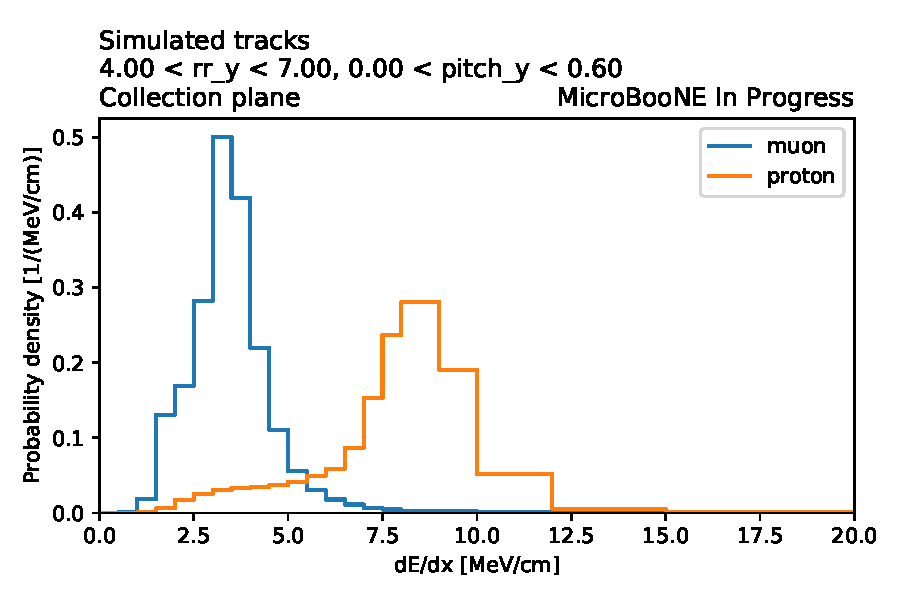
\includegraphics[width=1.00\textwidth]{llrpid/pdf_example_low_pitch.pdf}
    \end{subfigure}
    \begin{subfigure}[b]{0.48\textwidth}
    \centering
    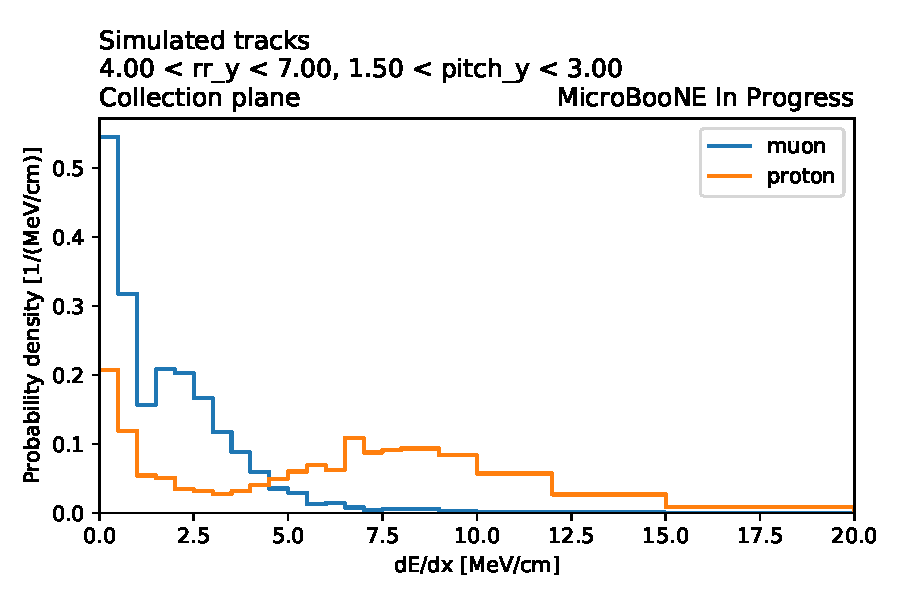
\includegraphics[width=1.00\textwidth]{llrpid/pdf_example_large_pitch.pdf}
    \end{subfigure}
\caption{Comparison of the expected distribution of \dedx for muons (blue) and protons (orange), for two different bins in residual range and pitch (left and right).}
\label{fig:llr_pid_pdf_example}
\end{center}
\end{figure}

For a given track, we consider the calorimetry objects on all three planes. 
For each plane, the \dedx, residual range, and pitch vectors are used to compute the likelihood of each particle type,
\[ \mathcal{L}(\text{type} | \text{plane}, dE/dx_{i = 1, ..., N},   \text{rr}_{i = 1, ..., N}, \text{pitch}_{i = 1, ..., N}) = \prod_{i=1}^N p(dE/dx_i | \text{type}, \text{plane}, \text{rr}_i, \text{pitch}_i) \]
where the index $i=1, ..., N$ runs over each hit for the considered plane.
The combination of the three planes happens in a straightforward way, by taking the product of the three likelihoods, or summing the log-likelihoods,
\[ p(dE/dx | \text{type}, \text{plane}, \text{rr}, \text{pitch}). \]
The likelihood ratio test statistic is chosen to perform the classification:
\[ T(dE/dx, \text{rr}, \text{pitch}) = \mathcal{L}(\text(muon)| dE/dx, \text{rr}, \text{pitch}) /  \mathcal{L}(\text(proton)| dE/dx, \text{rr}, \text{pitch}). \]
An example of the distribution of these variables, normalized between -1 and 1, is shown in Figure \ref{fig:llr_pid_uvy_example} for tracks contained within a fiducial volume, and backtracked to a muon, proton, or cosmic.

The likelihood ratio, as defined above, can be proven to be the most powerful statistical test, i.e. the one with the smallest mis-identification rate for any given value of the efficiency.
Any mis-modeling in the simulation used to build the likelihood produces a loss of power, as the test would not be the most powerful one.
Systematic uncertainties arise from the fact that the measured distribution of \dedx in the data may differ from the simulation, or because the properties of the tracks we consider, such as angular or length distributions, may not be properly simulated.
This behaviour is qualitatively present in all the PID methods.

\paragraph{Performance}
In a MC sample of contained protons and muons used to test the performance, this PID variable is able to reach 94\% muon efficiency, with a 10\% proton mis-ID rate.

A perhaps more interesting result is illustrated in Figure \ref{fig:llr_pid_uvy_example}.
This shows the distribution of the PID variable for tracks, with track score $>$ 0.5, that are reconstructed within 5 cm from the vertex, and well contained within the fiducial volume.
This is achieved by requiring that both the start and end points, after correcting for the SCE, are at least 20 cm farther away from each side of the TPC.
The plot shows how protons populate the left side of the distribution, whereas particles with smaller mass, like muons and pions populate the right side of the plot, and they are well separated around 0.
Tracks backtracked to cosmic rays are distributed along the whole spectrum, as, despite being mostly induced by muons, some of them are actually resulting from protons.
This tool shows the capability to distinguish proton-like from muon-like cosmic tracks.

\begin{figure}[H] 
    \centering
    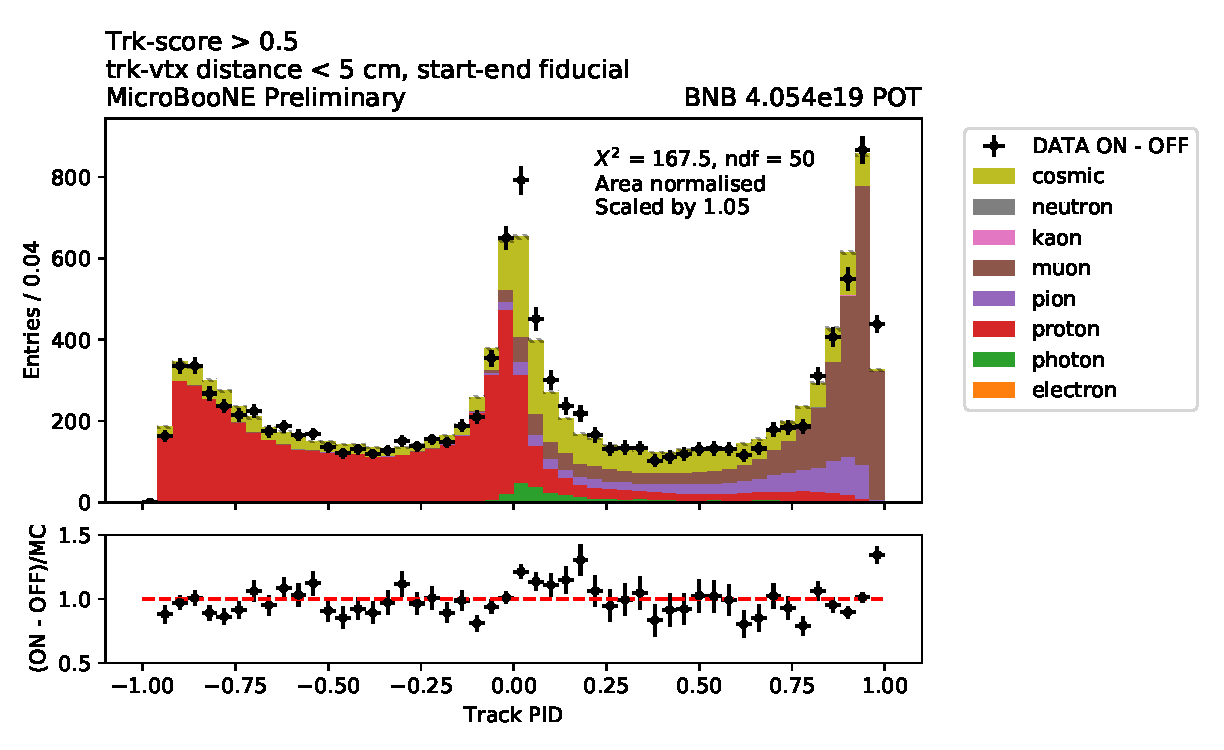
\includegraphics[width=1.0\textwidth]{llrpid/llr_012_n_area_norm.pdf}
    \caption{Distribution of the log-likelihood-ratio PID variable for neutrino-induced tracks well contained in the fiducial volume. This plot is produced by first normalising the data Beam OFF to the data Beam ON as usual. The Monte Carlo is weighted with the Genie spline and tune weights, and eventually area normalised to the subtraction Beam ON - Beam OFF. The scale factor for the simulation to obtain the area normalised comparison in this plot is 1.05.}
    \label{fig:llr_pid_uvy_example}
\end{figure}

Two more plots illustrate that using this particle identification method we are able to see the Bragg peak in the data as expected.
A selection of well contained tracks, defined similarly as before with track score $>$ 0.8 and pitch with respect to the collection plane $<$ 1 cm, is performed on the data Beam ON.
We show 2D histograms with values of \dedx vs residual range on the collection plane, for muon-like tracks with PID $>$ 0.5, and proton-like tracks with PID $<$ -0.5, on the left and right plots of Figure \ref{fig:llr_pid_pdf_example}, respectively.
The two different Bragg peaks are clearly visible and distinct from each other, due to the requirement on the track pitch.
The white bands show the theoretical prediction of the most probable value of the \dedx distribution in the range of pitch under consideration.
Remarkably, the core of the distribution sits along the white band, demonstrating good calorimetry reconstruction in the forward angular region.

\begin{figure}[H] 
\begin{center}
    \begin{subfigure}[b]{0.48\textwidth}
    \centering
    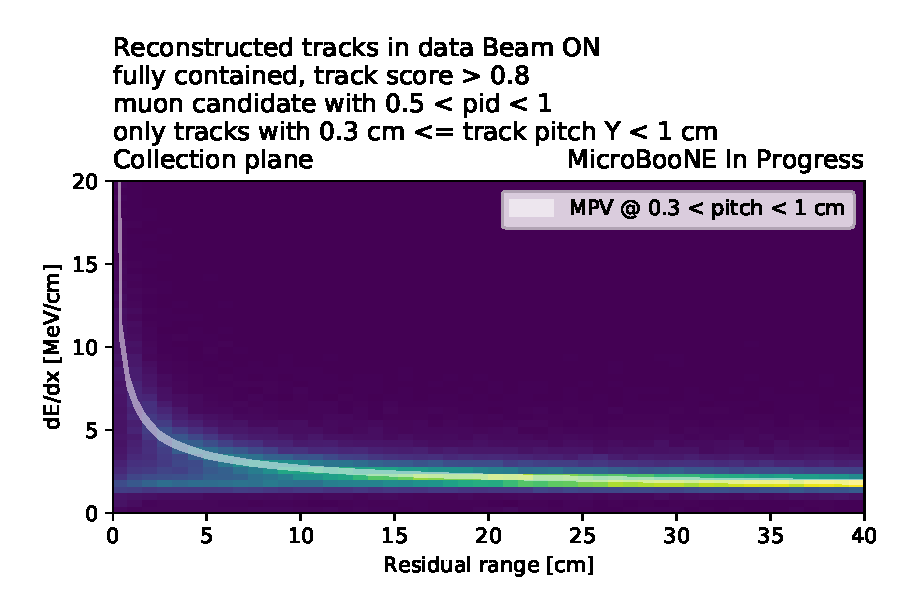
\includegraphics[width=1.00\textwidth]{llrpid/pdg_muon_03_pitch_10.pdf}
    \end{subfigure}
    \begin{subfigure}[b]{0.48\textwidth}
    \centering
    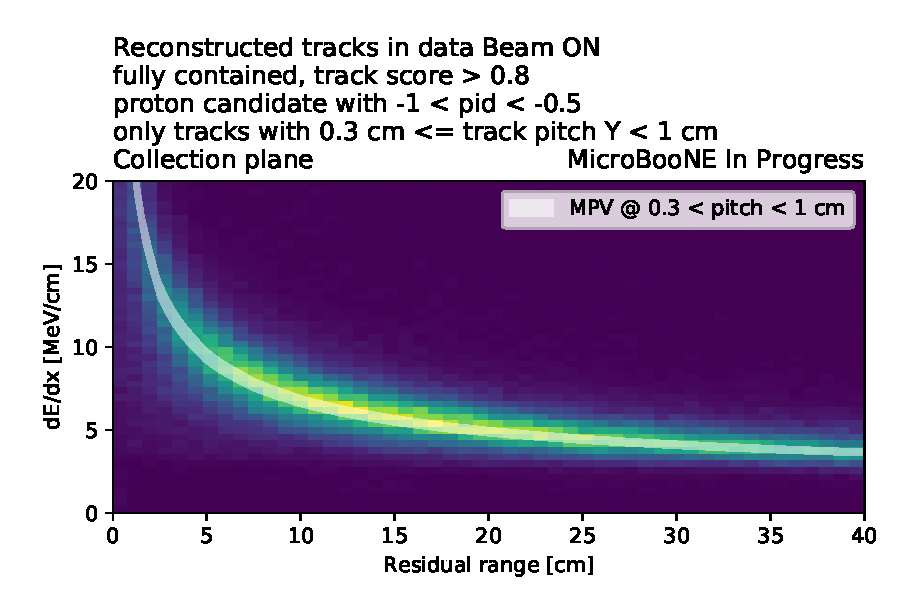
\includegraphics[width=1.00\textwidth]{llrpid/pdg_proton_03_pitch_10.pdf}
    \end{subfigure}
\caption{\dedx versus residual range on the collection plane for muon-like tracks (left) and proton-like tracks (right), as selected in the data Beam ON using the track PID.
The two Bragg peaks are clearly visible and distinct.
A white transparent band, superimposed on the distributions, shows the theoretical prediction for the most probable value, in the range of pitch considered in this plot, between 0.3 and 1 cm.
In the left plot, a component of MIP like particles at low residual range is clearly present.
This is due to the contamination of cosmic muons in the selected sample.}
\label{fig:llr_pid_pdf_example}
\end{center}
\end{figure}

The presence of the Bragg peak on the induction planes for protons at high pitch with respect to the collection plane has also been demonstrated, as shown in slide 26 of \cite{bib:calorimetry_collab_meeting}.

\subsubsection{$e$/$\gamma$ Separation}
\label{subsec:egammaspearation}


\par Distinguishing electron from photon EM-showers is one of the crucial steps required to perform a measurement of $\nu_e$ interactions in the BNB beam. Photon backgrounds to a $\nu_e$ measurement are largely caused by neutrino interactions with $\pi^0 \rightarrow \gamma\gamma$ in the final state; this topology dominates the $\nu_e$ event rate by approximately an order of magnitude. Three key features distinguish events with $\pi^0$ induced photon showers from $\nu_e$ interactions: (a) the presence of two final state EM showers, (b) the non-zero conversion distance separating the neutrino interaction vertex from the shower start point, and (c) the calorimetric separation via \dedx due to the overlapping ionization segment of $e^+$/$e^-$ pair-conversions through which most $\gamma$ showers manifest themselves. All three features are used in this analysis. In this section we describe briefly the use of these tools and demonstrate their performance with select plots from the $\nu_e$ high-energy sidedband described in detail in Sec.~\ref{sec:sidebands}.

\par \textbf{Two-shower requirement} Requiring a single reconstructed shower is the most straight-forward way to reject $\pi^0$ events. Figure~\ref{fig:nshowersdata} shows the discrimination of $\pi^0$ from $\nu_e$ events based on the number of showers at high energies. The dominant causes for remaining inefficiency in rejecting $\pi^0$s are highly-boosted $\pi^0$ decays, in which two aligned photons are merged into one shower, photons which go undetected, often low in energy (below 100 MeV) or because they escape the detector. While at high energy there is a sizeable fraction of $\nu_e$ events reconstructed with two showers in the final state (either because a true $\pi^0$ is produced or because of shower-splitting in the reconstruction) this is very rare at low energy and allows to require a single reconstructed shower in the final state in the analysis without impacting the efficiency at low energy.

\par \textbf{Track-shower distance} For events where hadronic activity at the neutrino interaction vertex is present, a clear gap between the vertex and the shower start-point can be used to reject $\gamma$ backgrounds. This is a powerful background mitigation tool in the 1$e$N$p$ $\nu_e$ selection. Two factors determine the performance of such a tool: the ability to detect protons and other hadronic activity at the vertex, and the accuracy with which the shower start-point is reconstructed. The shower start-point reconstruction accuracy determines the level of background rejection obtainable, as $\gamma$ showers lead to an exponential conversion-distance distribution. Figure~\ref{fig:tkshdistancedata} shows the separation power based on vertex displacement in the high-energy sideband. It is important to note that this background mitigation strategy is not applicable to single-electron searches, which are an important contribution to $\nu_e$ interactions, especially in the low-energy regime.

\begin{figure}[H] 
\begin{center}
    \begin{subfigure}[b]{0.45\textwidth}
    \centering
    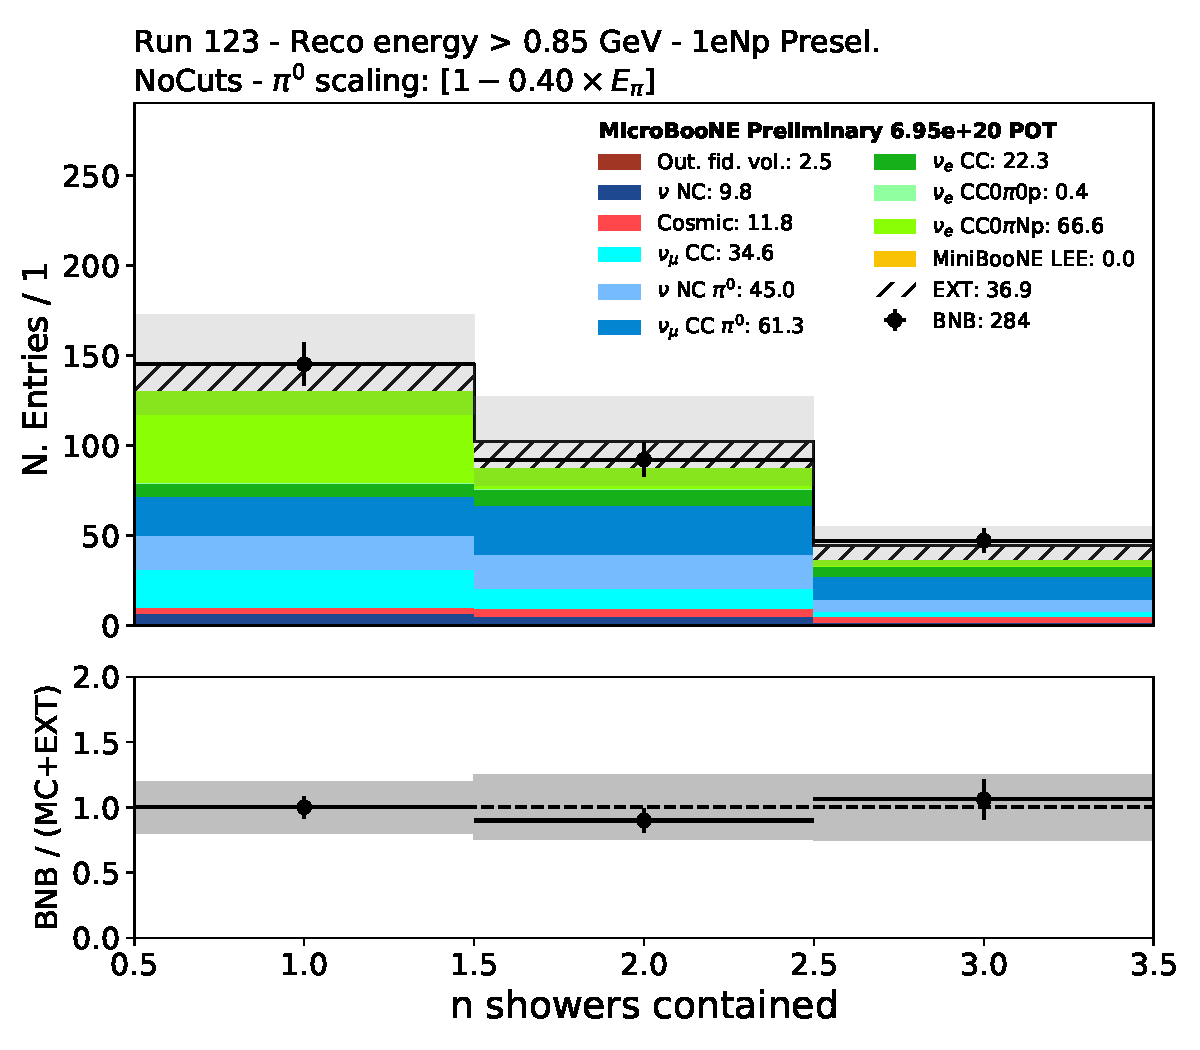
\includegraphics[width=1.00\textwidth]{egamma/n_showers_contained_run123_trkpid_lt_m01_tkshdistance_lt_10cm.pdf}
    \caption{\label{fig:nshowersdata} number of contained showers}
    \end{subfigure}
    \begin{subfigure}[b]{0.45\textwidth}
    \centering
    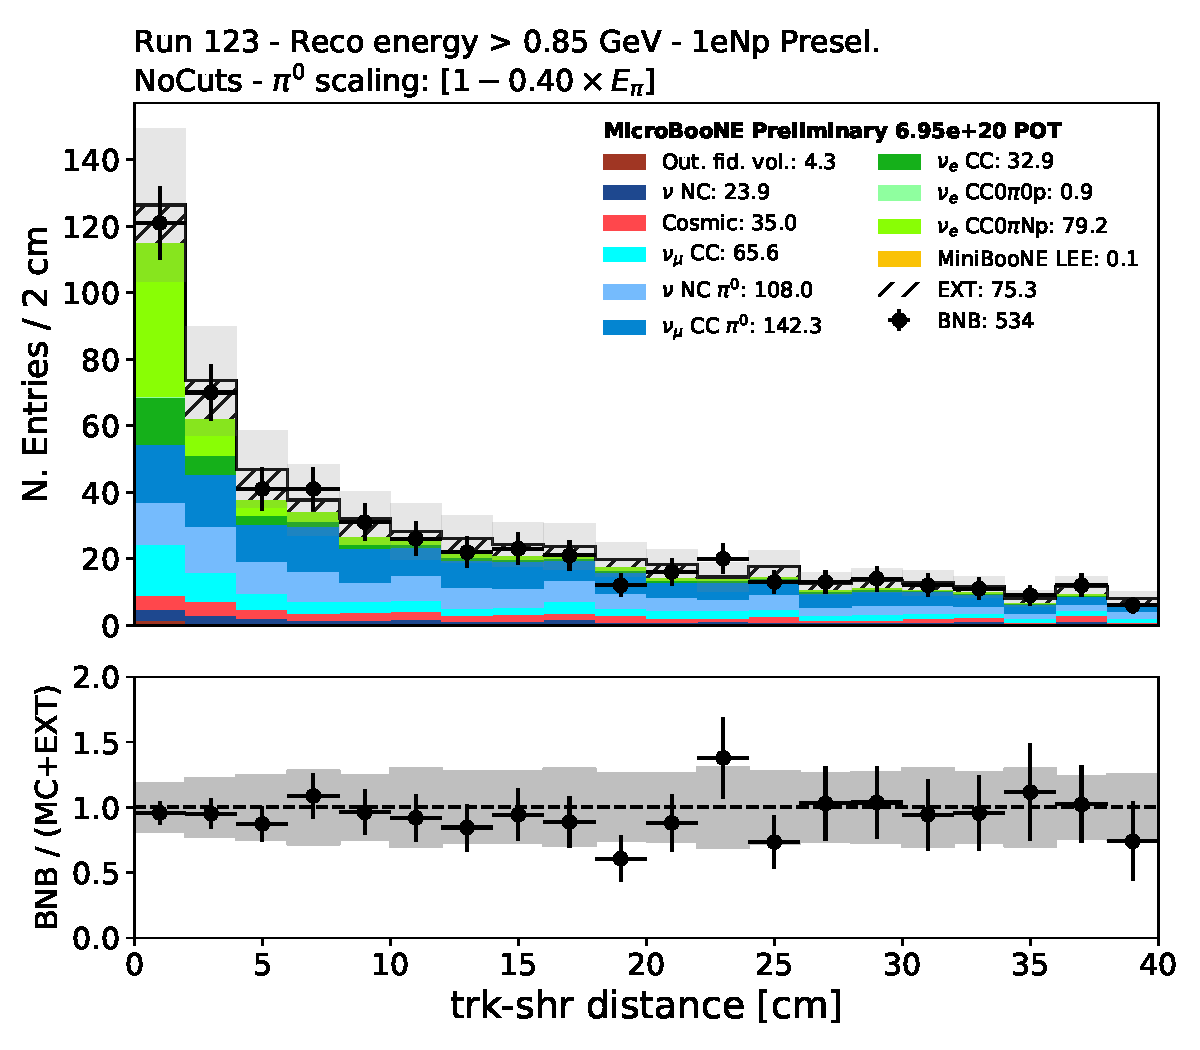
\includegraphics[width=1.00\textwidth]{egamma/tksh_distance_run123_trkpid_lt_m01.pdf}
    \caption{\label{fig:tkshdistancedata} 3D vertex displacement}
    \end{subfigure}
    \begin{subfigure}[b]{0.45\textwidth}
    \centering
    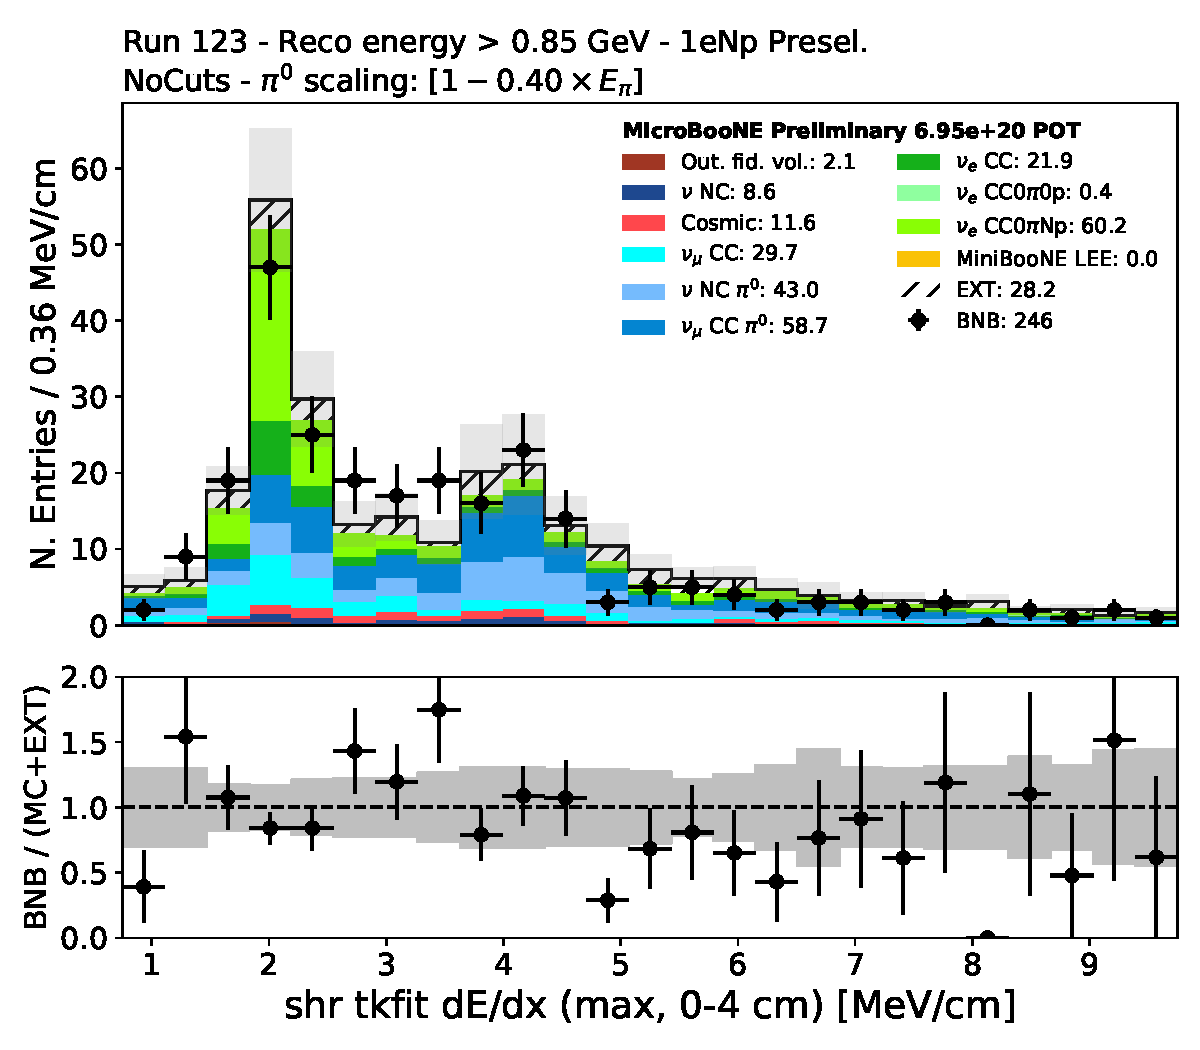
\includegraphics[width=1.00\textwidth]{egamma/shr_tkfit_dedx_max_run123_trkpid_lt_m01_tkshdistance_10cm.pdf}
    \caption{\label{fig:dedxdata:1enp} \dedx for \npsel events}
    \end{subfigure}
    \begin{subfigure}[b]{0.45\textwidth}
    \centering
    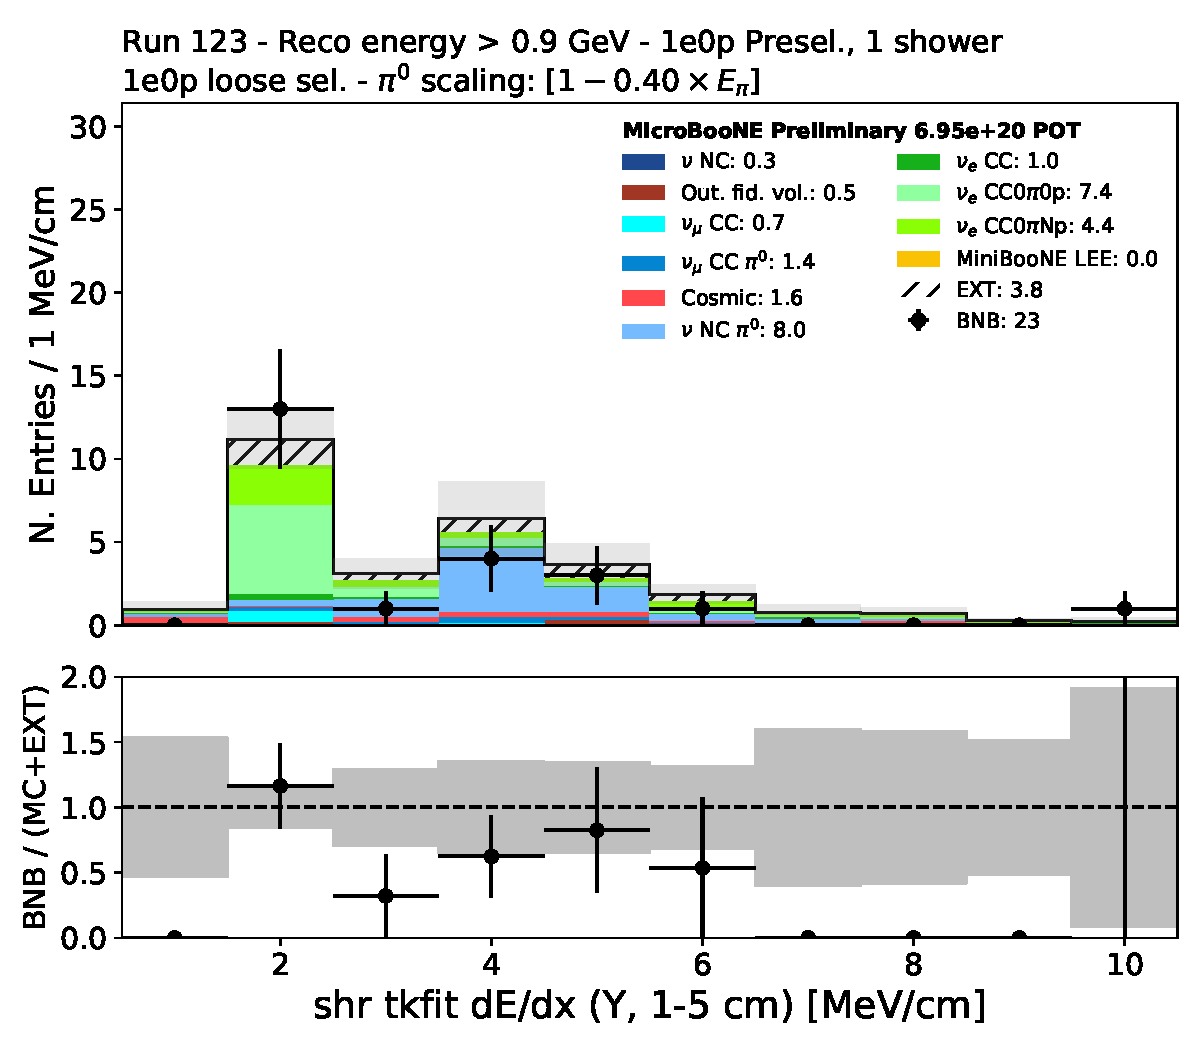
\includegraphics[width=1.00\textwidth]{1e0p/High_E_Sideband/loose_selection/shr_tkfit_gap10_dedx_Y.pdf}
    \caption{\label{fig:dedxdata:1e0p} \dedx for \zpsel events}
    \end{subfigure}
\caption{\label{fig:egammaseparationdata} Examples of  $e$/$\gamma$ separation from high-energy sidebands.}
\end{center}
\end{figure}

\par \textbf{Shower \dedx} The majority of photons manifest themselves in the TPC through the ionization released by the $e^+$/$e^-$ pair produced by pair-conversion. The electron-positron pair is highly aligned and overlaps on the mm-scale, leading to a doubly-ionizing charge-segment compared to electron showers. To measure this, we use the track fit of the main shower trunk and the calorimetric tools as loss, but accounting for local variations in the electric field. Figures~\ref{fig:dedxdata:1enp} and~\ref{fig:dedxdata:1e0p} shows the performance in $e$/$\gamma$ separation obtained in the high-energy sidebands for \npsel and \zpsel respectively. As can be seen in the figures, the main limitation to $e$/$\gamma$ separation via \dedx is the non-negligible fraction of photons reconstructed with a \dedx of less then 3 MeV/cm. This is due both to mis-reconstructed events, for which the start-point is incorrectly reconstructed by more than one or two cm, and to events where the photon shower's energy loss-profile is not as clearly distinguishable from that of a single electron. While the relative contribution of these two sources is still under determination, the second, an intrinsic feature of low-energy $\gamma$ showers rather than a reconstruction issue) can cause a significant mis-ID rate. For these showers, the production of a highly asymmetric electron-positron pair where one of the electrons is barely visible is more frequent. The impact of shower energy on the measured \dedx for a $\gamma$ shower is shown in figure~\ref{fig:dedxgammas:energy} where reconstructed calorimetric information is shown for truth-selected well reconstructed $\gamma$ showers. Below 100 MeV, where most $\gamma$ showers in the BNB are produced, the reconstructed \dedx is electron-like. The impact of distance from the shower start-point on whether \dedx is reconstructed to be 2 or 4 MeV/cm is also important, as can be seen in figure~\ref{fig:dedxgammas:dist}. This is particularly true for low-energy asymmetric pair-production events, and motivates utilizing \dedx information at different distances from the shower start-point for $e$/$\gamma$ separation. 



\begin{figure}[H] 
\begin{center}
    \begin{subfigure}[b]{0.45\textwidth}
    \centering
    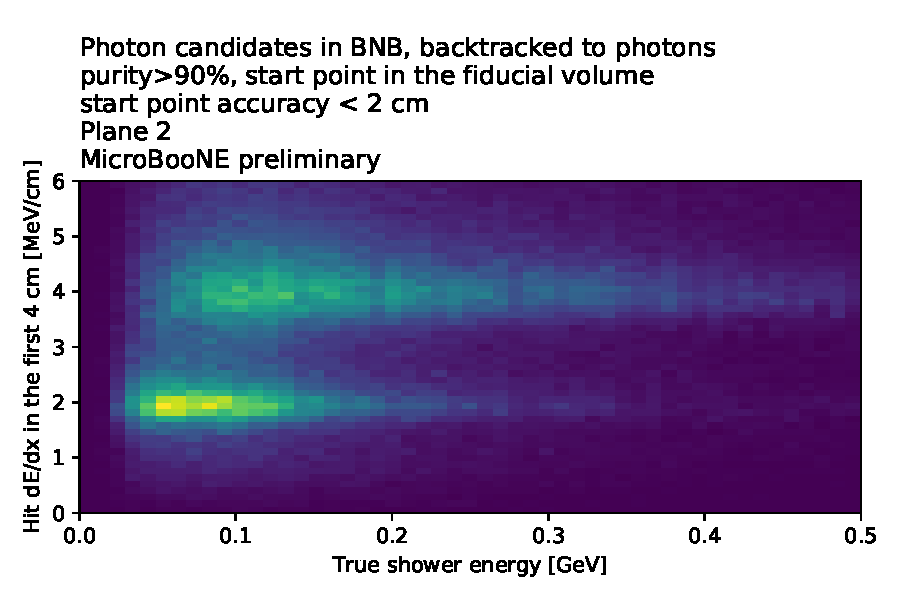
\includegraphics[width=1.00\textwidth]{egamma/plane2_photon_2d_dedx_sh_energy.pdf}
    \caption{\label{fig:dedxgammas:energy} \dedx vs. true $\gamma$ energy}
    \end{subfigure}
    \begin{subfigure}[b]{0.45\textwidth}
    \centering
    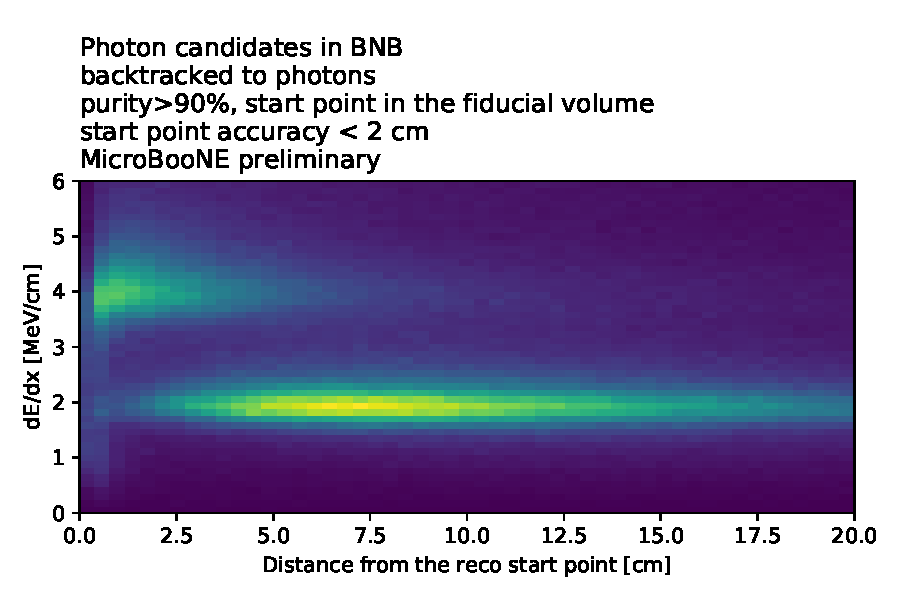
\includegraphics[width=1.00\textwidth]{egamma/photon_2d_dedx_dist.pdf}
    \caption{\label{fig:dedxgammas:dist} \dedx vs. distance from shower start for $\gamma$ showers}
    \end{subfigure}
\caption{\label{fig:dedxgammas} Impact of shower energy and distance from shower start on \dedx for  $\gamma$}
\end{center}
\end{figure}

Additional discriminating variables not described here which help enhance $e$/$\gamma$ separation and targer the recovery of reconstruction-related mis-ID are utilized in the analysis and presented in Sec.~\ref{sec:nueselection:inputs}.

%\newpage

\subsection{Energy Reconstruction}
\label{sec:ereco}
\par Energy reconstruction is performed through calorimetry for EM showers and through a measurement of a track's range for contained muons and protons. For muons (contained or uncontained), multiple Coulomb scattering (MCS) is also used to estimate the muon energy. The energy resolution obtained for different particles is reported in Table~\ref{tab:eres}. More information on each particle's energy resolution is reported in Figure~\ref{fig:eres:particle} where the reconstructed vs. true energy distribution (in log-scale) is shown on the left, next to a plot of energy resolution vs. true energy on the right. The energy resolution reported here is obtained from a Gaussian plus one-sided exponential fit to the distribution $[E_{\rm reco}-E_{\rm true}] / E_{\rm true}$; see Figure \ref{fig:eres:elec:binned}. The resolution reported refers only to the Gaussian width $\sigma$ extracted in the fit, and therefore does not account for tails, which are significant in the case of EM shower energy reconstruction, and described below.


\begin{table}[H]
\centering
  \begin{tabular}{ | c | c |  }
    \hline
    particle & kinetic energy resolution  \\ \hline
    proton & 4\% at 100 MeV, 1\% at 200 MeV \\ \hline
    muon (range) & 3\%  \\ \hline
    muon (MCS) & 25\% at 100 MeV, $< 10$\% above 400 MeV  \\ \hline
    electron & 15\%  \\
    \hline
    
  \end{tabular}
  \caption{\label{tab:eres} Energy resolution for different particle species.}
 \end{table}
 
 \par For EM showers, the calorimetric energy reconstruction response has a significant non-Gaussian component, as well as a large bias. Both effects are attributable to reconstruction effects associated with the under-clustering of charge. The energy bias is found to be of order 20\% approximately flat in energy, and motivates a definition of a corrected shower energy, defined as $E_{\rm corrected} = E_{\rm calorimetry} / 0.83$, derived from truth-studies of electron showers from $\nu_e$ interactions. The non-Gaussian response for EM energy reconstruction can be modeled through a Gaussian plus one-sided exponential distribution. Figure~\ref{fig:eres:elec:binned} shows, in different bins of true energy, the fractional energy response and a fit to a Gaussian plus one-sided exponential function. The residual energy bias, after the 20\% correction applied, is of order $3-8$\% depending on the bin, as denoted by the $\mu$ term reported in each plot. 
 
\begin{figure}[ht]
\begin{center}
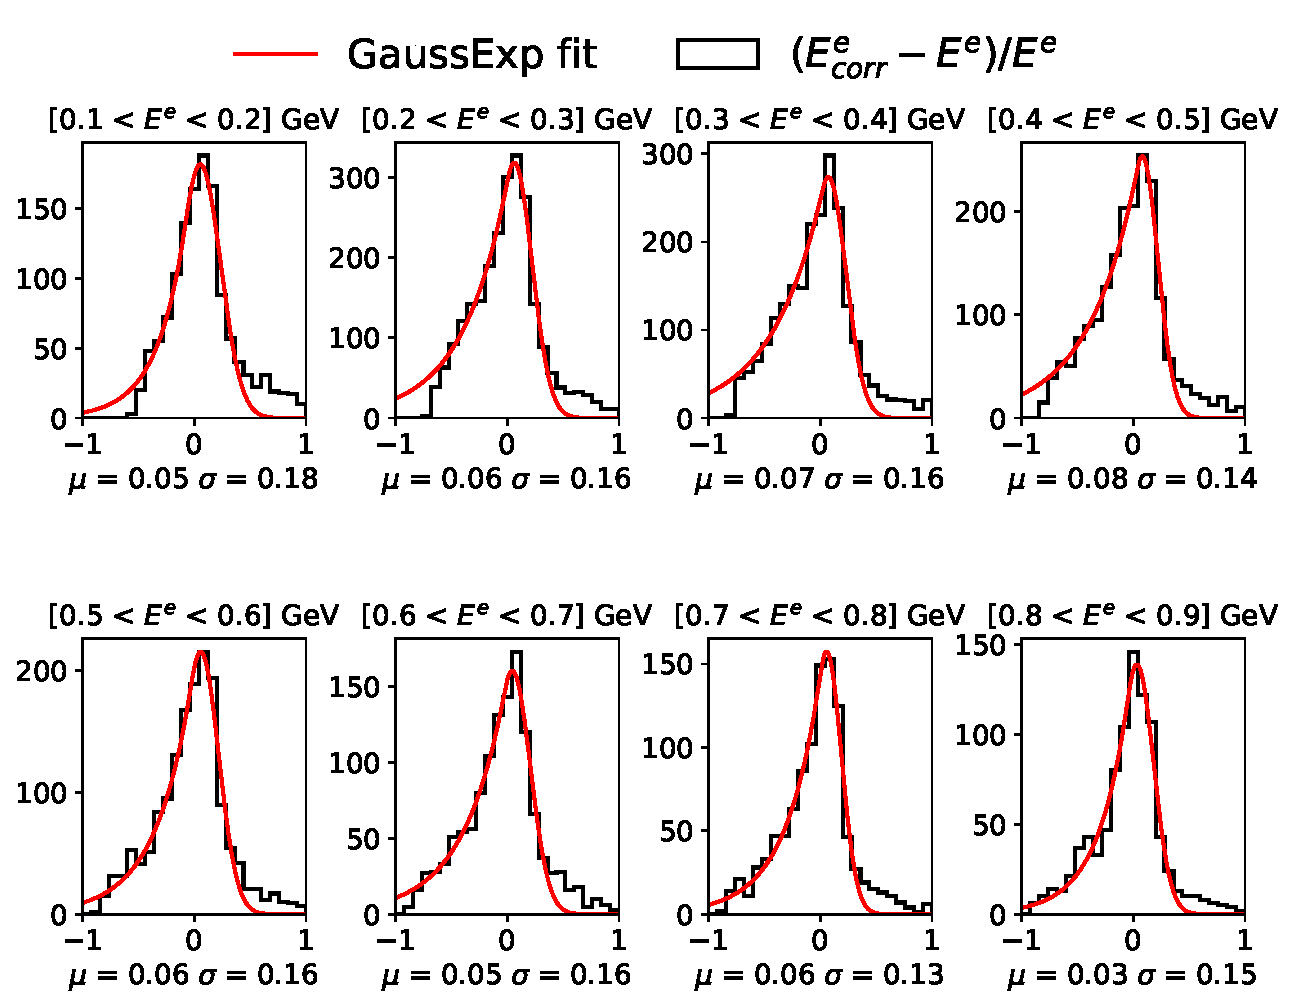
\includegraphics[width=0.75\textwidth]{ereco/elec_eres_binned.pdf}
\caption{\label{fig:eres:elec:binned}Energy resolution for electron showers.}
\end{center}
\end{figure}
 
\clearpage

\begin{figure}[H] 
\begin{center}
    \begin{subfigure}[b]{0.4\textwidth}
    \centering
    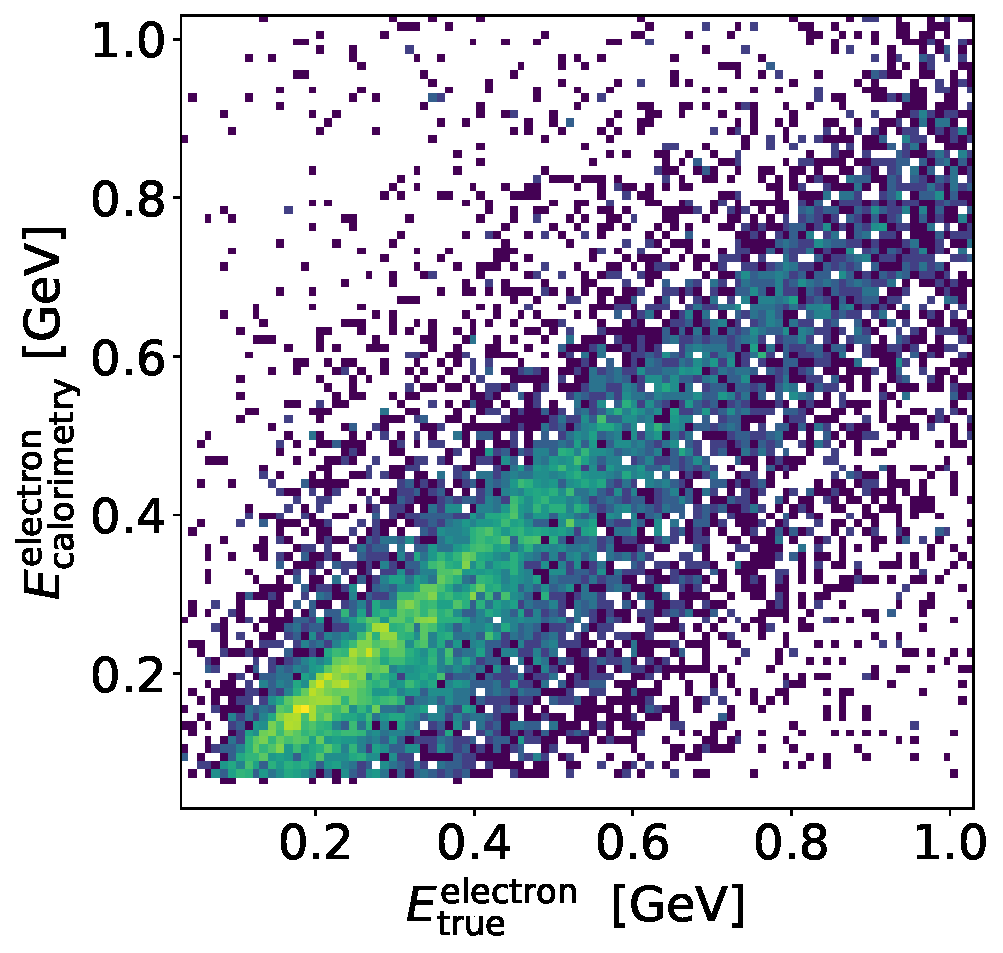
\includegraphics[width=1.00\textwidth]{ereco/electron_eres2D.pdf}
    %\caption{\label{fig:eres:elec:2d} }
    \end{subfigure}
    \begin{subfigure}[b]{0.38\textwidth}
    \centering
    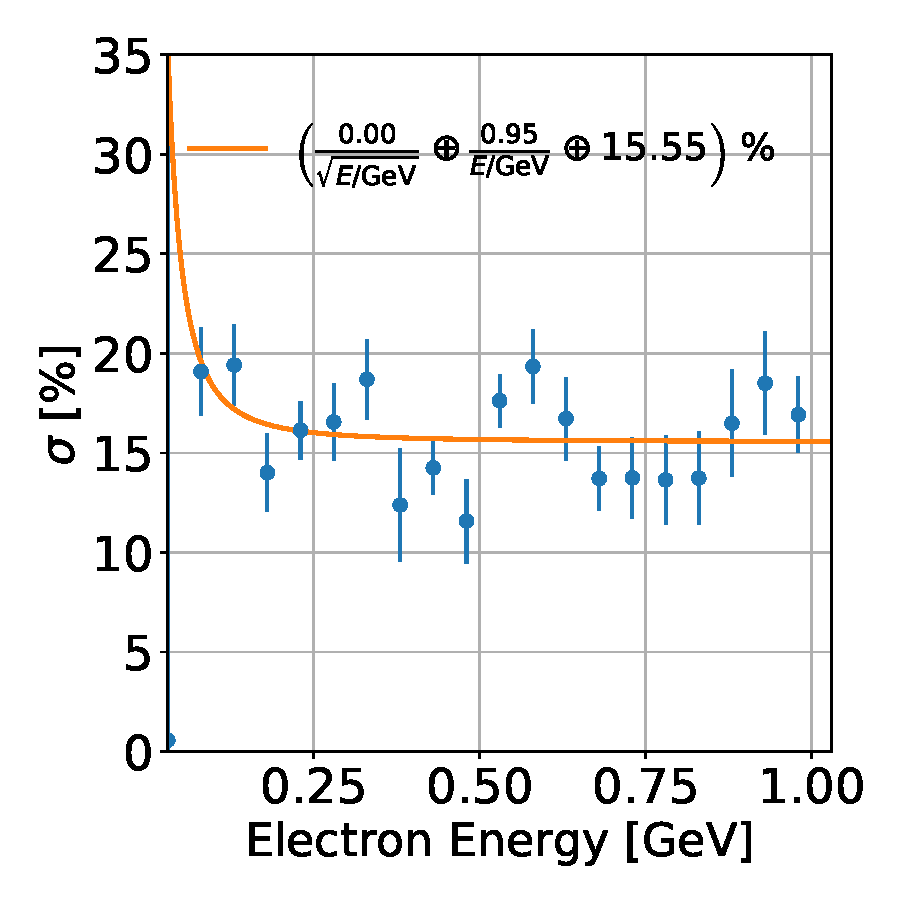
\includegraphics[width=1.00\textwidth]{ereco/elec_eres_vs_true.pdf}
    %\caption{\label{fig:eres:elec:vstrue} }
    \end{subfigure}
    \begin{subfigure}[b]{0.4\textwidth}
    \centering
    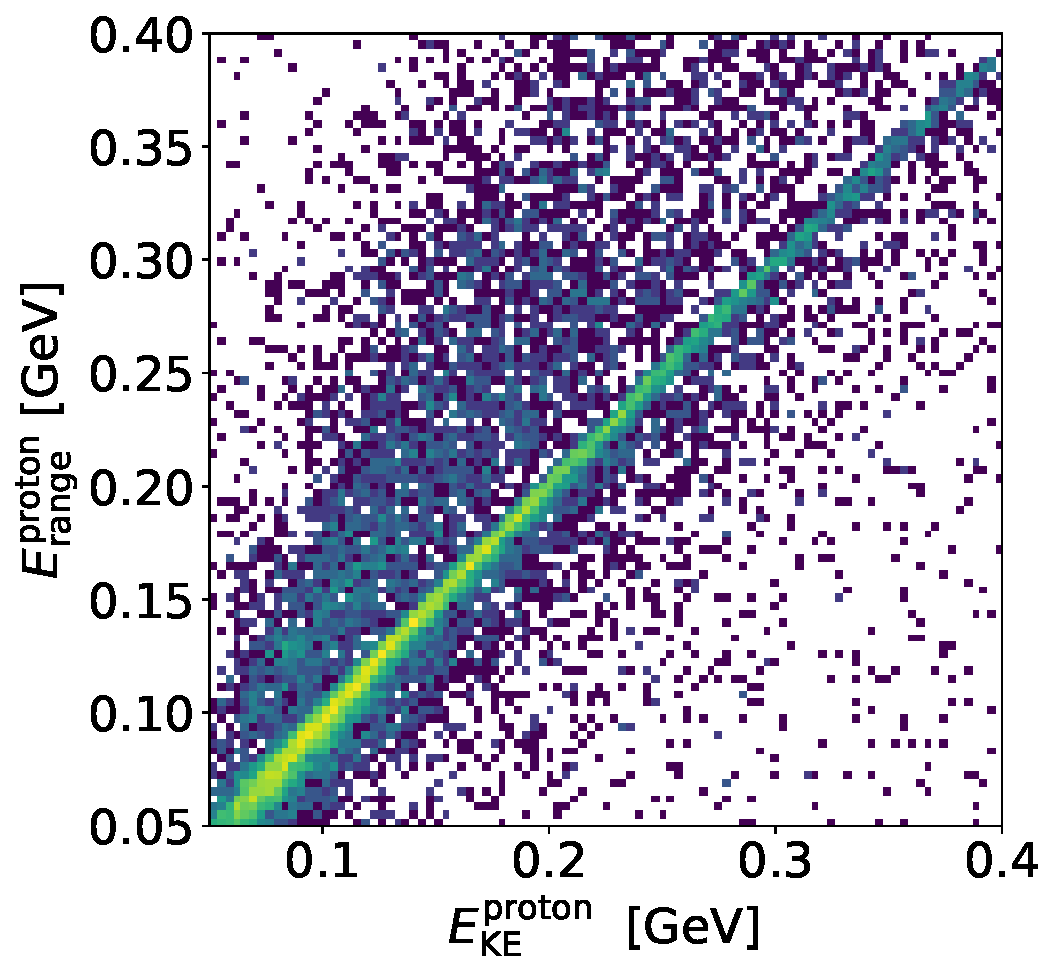
\includegraphics[width=1.00\textwidth]{ereco/proton_eres2D.pdf}
    %\caption{\label{fig:eres:proton:2d} }
    \end{subfigure}
    \begin{subfigure}[b]{0.38\textwidth}
    \centering
    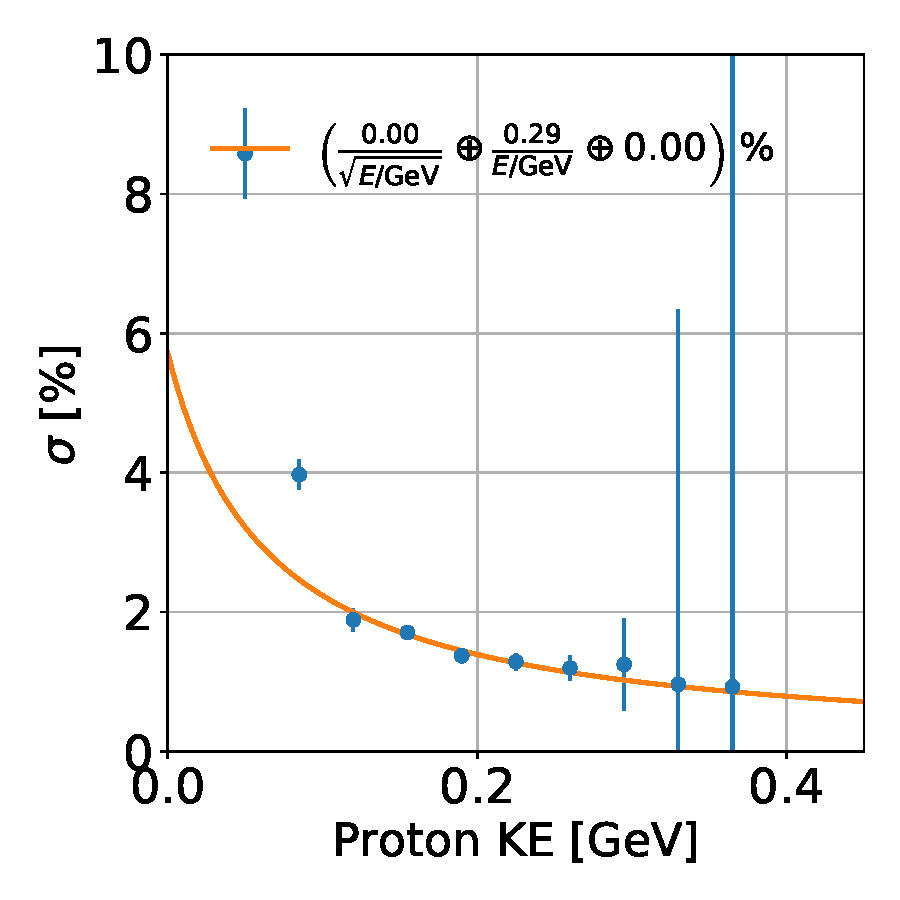
\includegraphics[width=1.00\textwidth]{ereco/proton_eres_vs_true.pdf}
    %\caption{\label{fig:eres:proton:vstrue} }
    \end{subfigure}
    \begin{subfigure}[b]{0.4\textwidth}
    \centering
    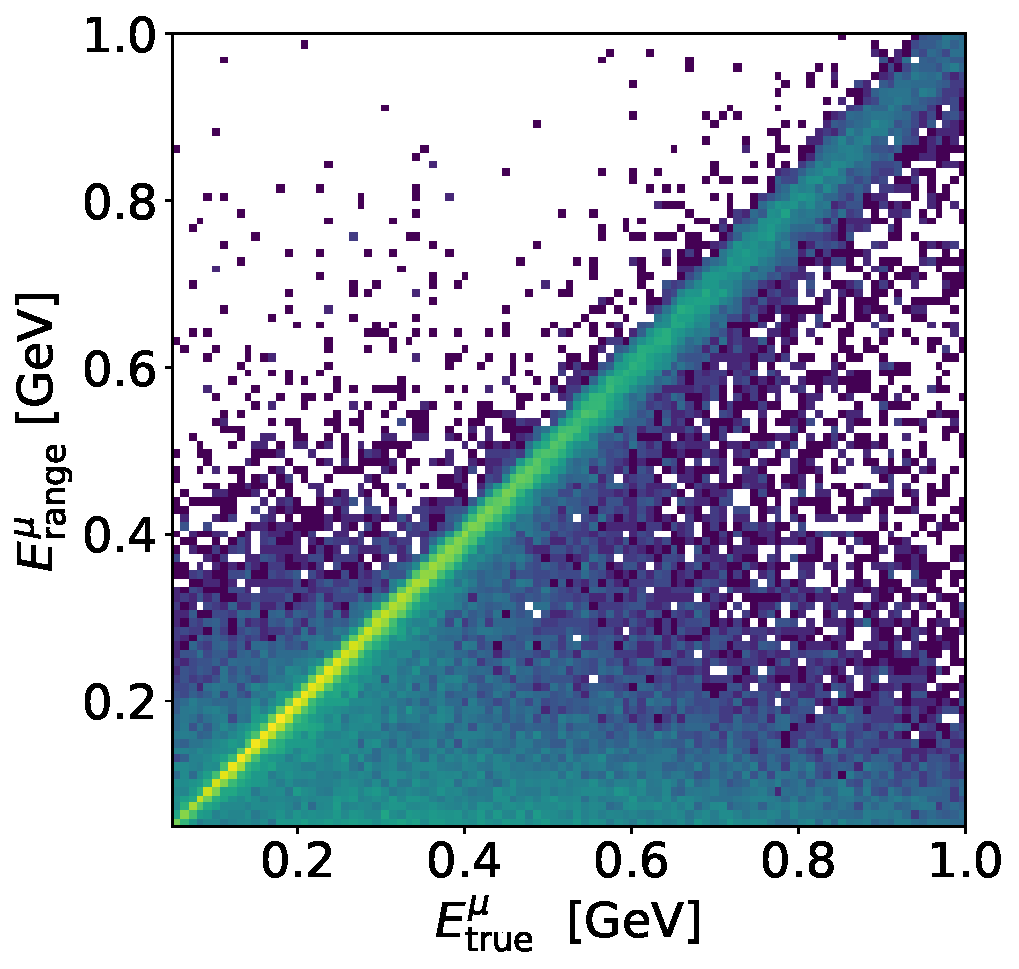
\includegraphics[width=1.00\textwidth]{ereco/muon_range_eres2D.pdf}
    %\caption{\label{fig:eres:muon:2d} }
    \end{subfigure}
    \begin{subfigure}[b]{0.38\textwidth}
    \centering
    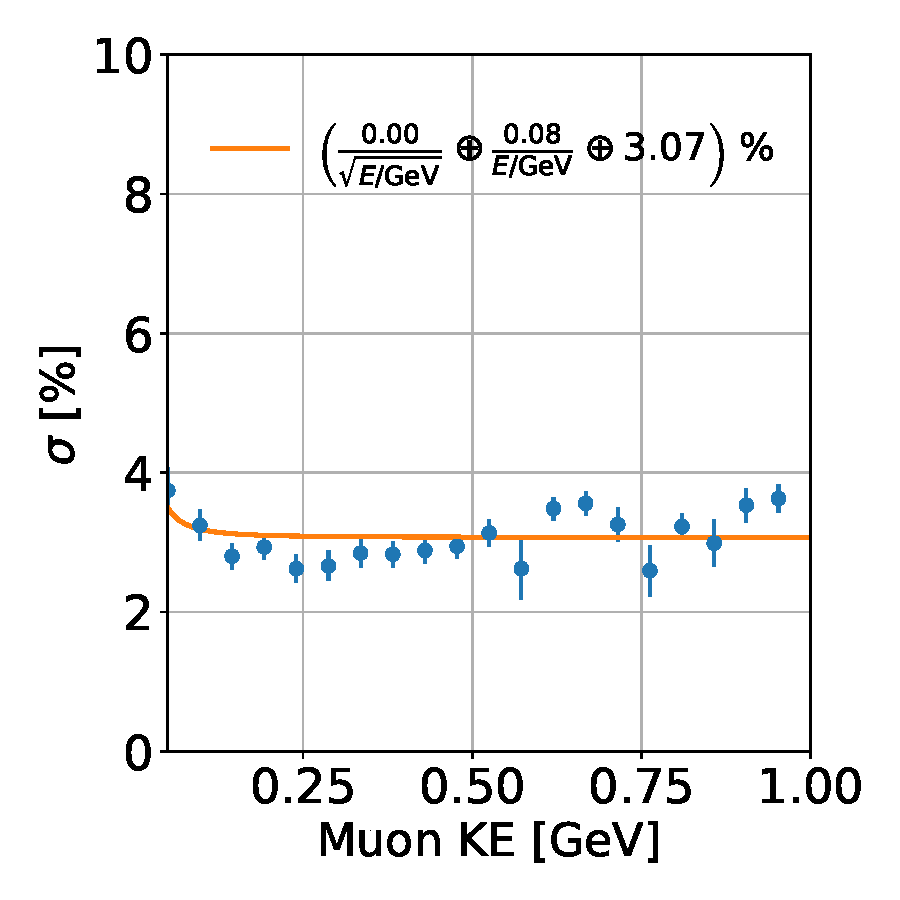
\includegraphics[width=1.00\textwidth]{ereco/muon_range_eres_vs_true.pdf}
    %\caption{\label{fig:eres:muon:vstrue} }
    \end{subfigure}
\caption{\label{fig:eres:particle}Energy resolution for electrons (top), protons (center) and muons (bottom). Left: reconstructed vs. true energy resolution (log-scale). Right: energy resolution from Gaussian fit to $[E_{\rm reco}-E_{\rm true}] / E_{\rm true}$.}
\end{center}
\end{figure}

\subsubsection{Neutrino Energy Reconstruction}

\par In this analysis, the energy reconstruction for neutrino interactions is performed through a sum of the visible energy of the various reconstructed final-state particles in the interaction. For $\nu_e$ events in the \zpsel and \npsel, the reconstructed energy is defined as:
\begin{equation}
    E_{\rm reco}^{\nu_e} = E_{\rm corrected}^{\rm electron} + \sum_{\rm tracks} E_{\rm range}^{\rm proton}.
\end{equation}{}
For contained $\nu_{\mu}$ interactions, the reconstructed energy is defined as:

\begin{equation}
    E_{\rm reco}^{\nu_{\mu}} = E_{\rm range}^{\rm muon} + \sum_{\rm protons} E_{\rm range}^{\rm proton} + 0.105 \; GeV
\end{equation}{}

Figure~\ref{fig:eres:neutrino} shows the comparison between reconstructed energy and truth visible energy, which is defined as the sum of the lepton energy, pion energy (if present), and proton energy (for all protons above 40 MeV of KE). This comparison shows very accurate energy reconstruction for most $\nu_{\mu}$ events. For $\nu_e$ interactions the energy resolution is on average less accurate, with smearing dominated by the worse energy resolution of electron showers.

\begin{figure}[H] 
\begin{center}
    \begin{subfigure}[b]{0.4\textwidth}
    \centering
    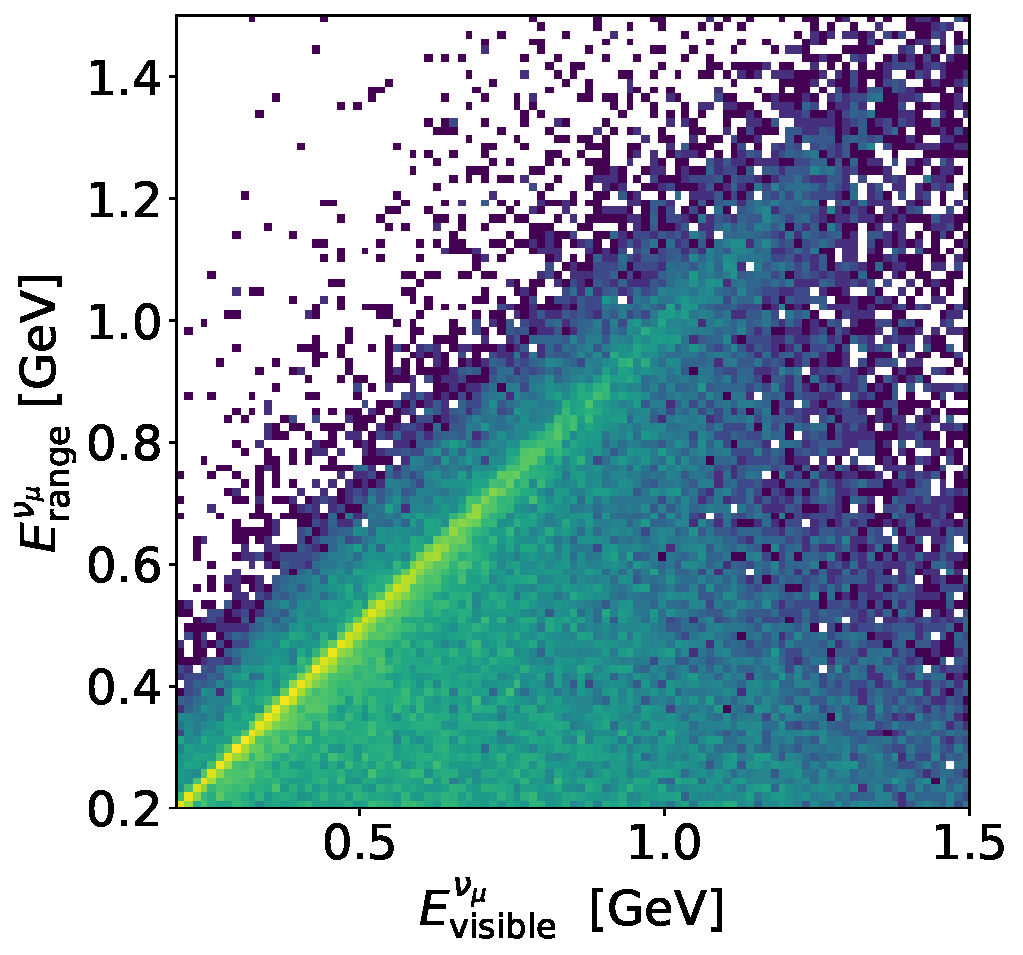
\includegraphics[width=1.00\textwidth]{ereco/numu_energy_visible_eres2D.pdf}
    \caption{\label{fig:eres:numu:2d} Muon nueutrinos. }
    \end{subfigure}
    \begin{subfigure}[b]{0.4\textwidth}
    \centering
    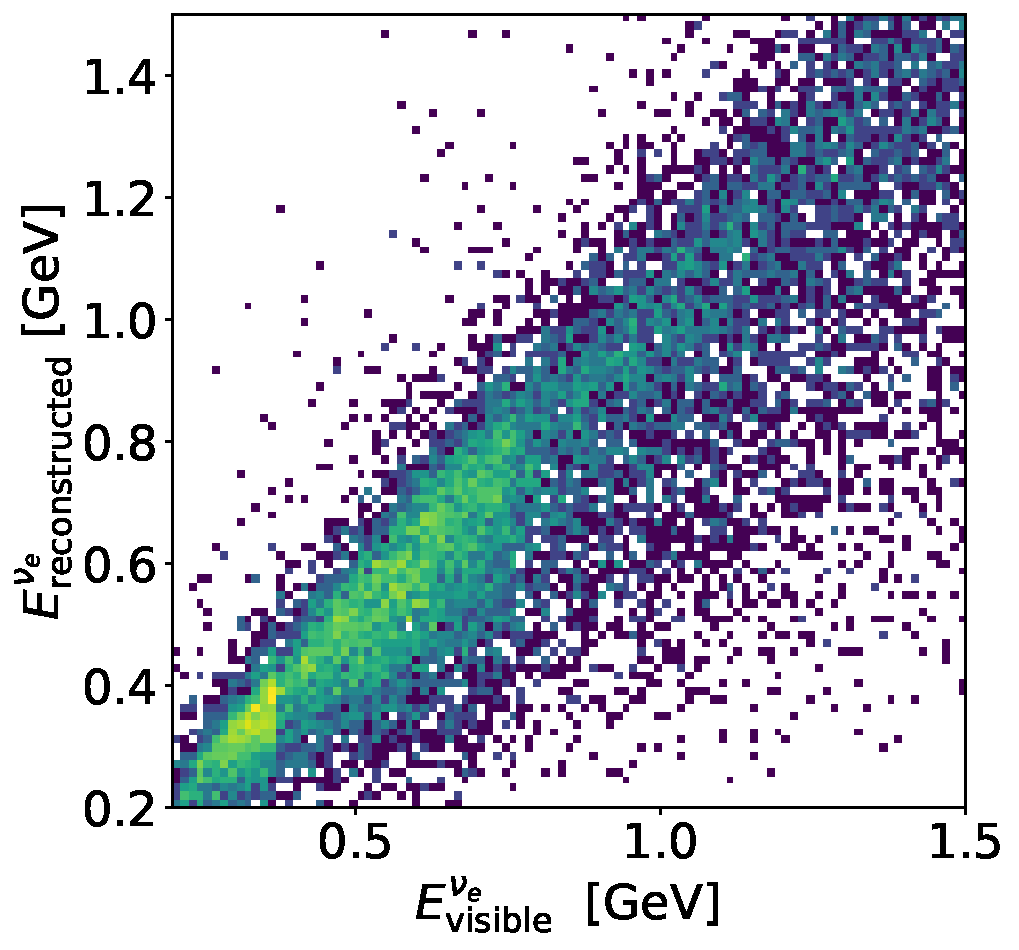
\includegraphics[width=1.00\textwidth]{ereco/nue_visible_eres2D.pdf}
    \caption{\label{fig:eres:nue:vstrue} Electron neutrinos.}
    \end{subfigure}
\caption{\label{fig:eres:neutrino}Log-scale color-maps of reconstructed vs. true energy. On the $\nu_e$ side the vertical features observed are a consequence of the different samples  and their statistics.}
\end{center}
\end{figure}
